% Options for packages loaded elsewhere
\PassOptionsToPackage{unicode}{hyperref}
\PassOptionsToPackage{hyphens}{url}
%
\documentclass[
]{article}
\usepackage{amsmath,amssymb}
\usepackage{iftex}
\ifPDFTeX
  \usepackage[T1]{fontenc}
  \usepackage[utf8]{inputenc}
  \usepackage{textcomp} % provide euro and other symbols
\else % if luatex or xetex
  \usepackage{unicode-math} % this also loads fontspec
  \defaultfontfeatures{Scale=MatchLowercase}
  \defaultfontfeatures[\rmfamily]{Ligatures=TeX,Scale=1}
\fi
\usepackage{lmodern}
\ifPDFTeX\else
  % xetex/luatex font selection
\fi
% Use upquote if available, for straight quotes in verbatim environments
\IfFileExists{upquote.sty}{\usepackage{upquote}}{}
\IfFileExists{microtype.sty}{% use microtype if available
  \usepackage[]{microtype}
  \UseMicrotypeSet[protrusion]{basicmath} % disable protrusion for tt fonts
}{}
\makeatletter
\@ifundefined{KOMAClassName}{% if non-KOMA class
  \IfFileExists{parskip.sty}{%
    \usepackage{parskip}
  }{% else
    \setlength{\parindent}{0pt}
    \setlength{\parskip}{6pt plus 2pt minus 1pt}}
}{% if KOMA class
  \KOMAoptions{parskip=half}}
\makeatother
\usepackage{xcolor}
\usepackage[margin=1in]{geometry}
\usepackage{color}
\usepackage{fancyvrb}
\newcommand{\VerbBar}{|}
\newcommand{\VERB}{\Verb[commandchars=\\\{\}]}
\DefineVerbatimEnvironment{Highlighting}{Verbatim}{commandchars=\\\{\}}
% Add ',fontsize=\small' for more characters per line
\usepackage{framed}
\definecolor{shadecolor}{RGB}{248,248,248}
\newenvironment{Shaded}{\begin{snugshade}}{\end{snugshade}}
\newcommand{\AlertTok}[1]{\textcolor[rgb]{0.94,0.16,0.16}{#1}}
\newcommand{\AnnotationTok}[1]{\textcolor[rgb]{0.56,0.35,0.01}{\textbf{\textit{#1}}}}
\newcommand{\AttributeTok}[1]{\textcolor[rgb]{0.13,0.29,0.53}{#1}}
\newcommand{\BaseNTok}[1]{\textcolor[rgb]{0.00,0.00,0.81}{#1}}
\newcommand{\BuiltInTok}[1]{#1}
\newcommand{\CharTok}[1]{\textcolor[rgb]{0.31,0.60,0.02}{#1}}
\newcommand{\CommentTok}[1]{\textcolor[rgb]{0.56,0.35,0.01}{\textit{#1}}}
\newcommand{\CommentVarTok}[1]{\textcolor[rgb]{0.56,0.35,0.01}{\textbf{\textit{#1}}}}
\newcommand{\ConstantTok}[1]{\textcolor[rgb]{0.56,0.35,0.01}{#1}}
\newcommand{\ControlFlowTok}[1]{\textcolor[rgb]{0.13,0.29,0.53}{\textbf{#1}}}
\newcommand{\DataTypeTok}[1]{\textcolor[rgb]{0.13,0.29,0.53}{#1}}
\newcommand{\DecValTok}[1]{\textcolor[rgb]{0.00,0.00,0.81}{#1}}
\newcommand{\DocumentationTok}[1]{\textcolor[rgb]{0.56,0.35,0.01}{\textbf{\textit{#1}}}}
\newcommand{\ErrorTok}[1]{\textcolor[rgb]{0.64,0.00,0.00}{\textbf{#1}}}
\newcommand{\ExtensionTok}[1]{#1}
\newcommand{\FloatTok}[1]{\textcolor[rgb]{0.00,0.00,0.81}{#1}}
\newcommand{\FunctionTok}[1]{\textcolor[rgb]{0.13,0.29,0.53}{\textbf{#1}}}
\newcommand{\ImportTok}[1]{#1}
\newcommand{\InformationTok}[1]{\textcolor[rgb]{0.56,0.35,0.01}{\textbf{\textit{#1}}}}
\newcommand{\KeywordTok}[1]{\textcolor[rgb]{0.13,0.29,0.53}{\textbf{#1}}}
\newcommand{\NormalTok}[1]{#1}
\newcommand{\OperatorTok}[1]{\textcolor[rgb]{0.81,0.36,0.00}{\textbf{#1}}}
\newcommand{\OtherTok}[1]{\textcolor[rgb]{0.56,0.35,0.01}{#1}}
\newcommand{\PreprocessorTok}[1]{\textcolor[rgb]{0.56,0.35,0.01}{\textit{#1}}}
\newcommand{\RegionMarkerTok}[1]{#1}
\newcommand{\SpecialCharTok}[1]{\textcolor[rgb]{0.81,0.36,0.00}{\textbf{#1}}}
\newcommand{\SpecialStringTok}[1]{\textcolor[rgb]{0.31,0.60,0.02}{#1}}
\newcommand{\StringTok}[1]{\textcolor[rgb]{0.31,0.60,0.02}{#1}}
\newcommand{\VariableTok}[1]{\textcolor[rgb]{0.00,0.00,0.00}{#1}}
\newcommand{\VerbatimStringTok}[1]{\textcolor[rgb]{0.31,0.60,0.02}{#1}}
\newcommand{\WarningTok}[1]{\textcolor[rgb]{0.56,0.35,0.01}{\textbf{\textit{#1}}}}
\usepackage{longtable,booktabs,array}
\usepackage{calc} % for calculating minipage widths
% Correct order of tables after \paragraph or \subparagraph
\usepackage{etoolbox}
\makeatletter
\patchcmd\longtable{\par}{\if@noskipsec\mbox{}\fi\par}{}{}
\makeatother
% Allow footnotes in longtable head/foot
\IfFileExists{footnotehyper.sty}{\usepackage{footnotehyper}}{\usepackage{footnote}}
\makesavenoteenv{longtable}
\usepackage{graphicx}
\makeatletter
\def\maxwidth{\ifdim\Gin@nat@width>\linewidth\linewidth\else\Gin@nat@width\fi}
\def\maxheight{\ifdim\Gin@nat@height>\textheight\textheight\else\Gin@nat@height\fi}
\makeatother
% Scale images if necessary, so that they will not overflow the page
% margins by default, and it is still possible to overwrite the defaults
% using explicit options in \includegraphics[width, height, ...]{}
\setkeys{Gin}{width=\maxwidth,height=\maxheight,keepaspectratio}
% Set default figure placement to htbp
\makeatletter
\def\fps@figure{htbp}
\makeatother
\setlength{\emergencystretch}{3em} % prevent overfull lines
\providecommand{\tightlist}{%
  \setlength{\itemsep}{0pt}\setlength{\parskip}{0pt}}
\setcounter{secnumdepth}{-\maxdimen} % remove section numbering
\ifLuaTeX
  \usepackage{selnolig}  % disable illegal ligatures
\fi
\usepackage{bookmark}
\IfFileExists{xurl.sty}{\usepackage{xurl}}{} % add URL line breaks if available
\urlstyle{same}
\hypersetup{
  pdftitle={Curso de Especialização em Data Science e Estatística Aplicada},
  pdfauthor={Ana Maria Alves da Silva},
  hidelinks,
  pdfcreator={LaTeX via pandoc}}

\title{Curso de Especialização em Data Science e Estatística Aplicada}
\author{Ana Maria Alves da Silva}
\date{2024-06-04}

\begin{document}
\maketitle

\emph{Questão 1. Na ferramenta SQLite IDE, crie e execute os scripts do
BD disponíveis em
\href{https://docs.google.com/document/d/1_ebLMDXezQl8xBTJn7a9LKbeIsNTbvIEYxSeqMuZbhc/edit?usp=drive_link}{google
drive}.}

\subsubsection{Solução:}\label{soluuxe7uxe3o}

\begin{itemize}
\tightlist
\item
  Passo 1: Criar as tabelas.
\end{itemize}

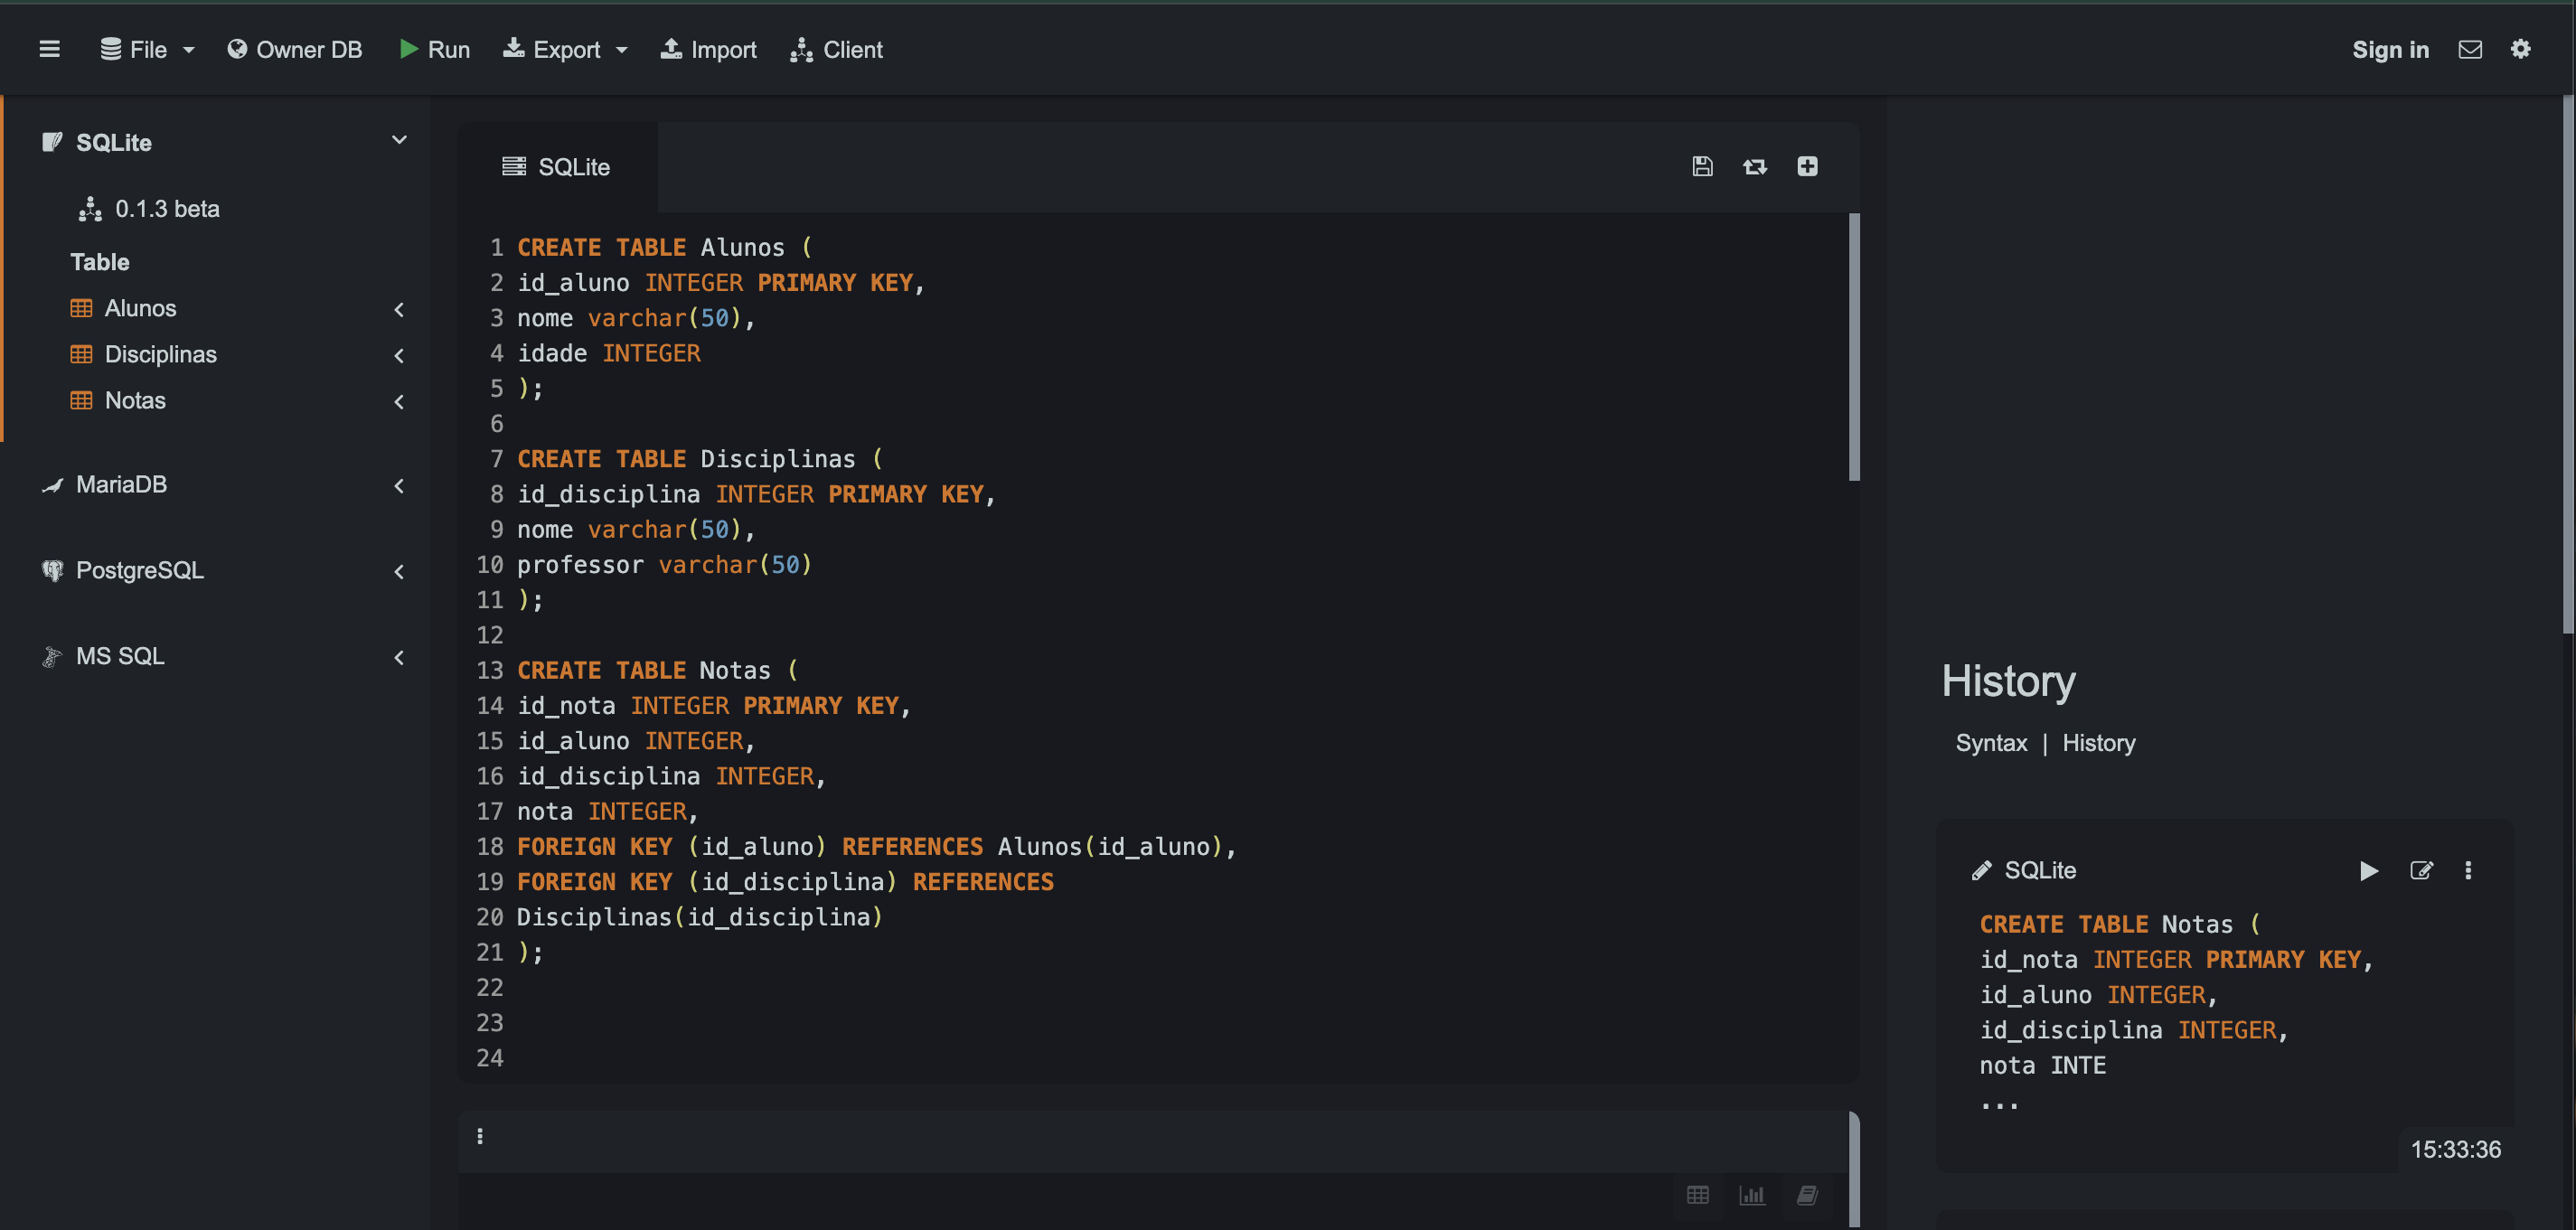
\includegraphics{create_table.png}

\begin{itemize}
\tightlist
\item
  Passo 2: Inserir dados na tabela Alunos.
\end{itemize}

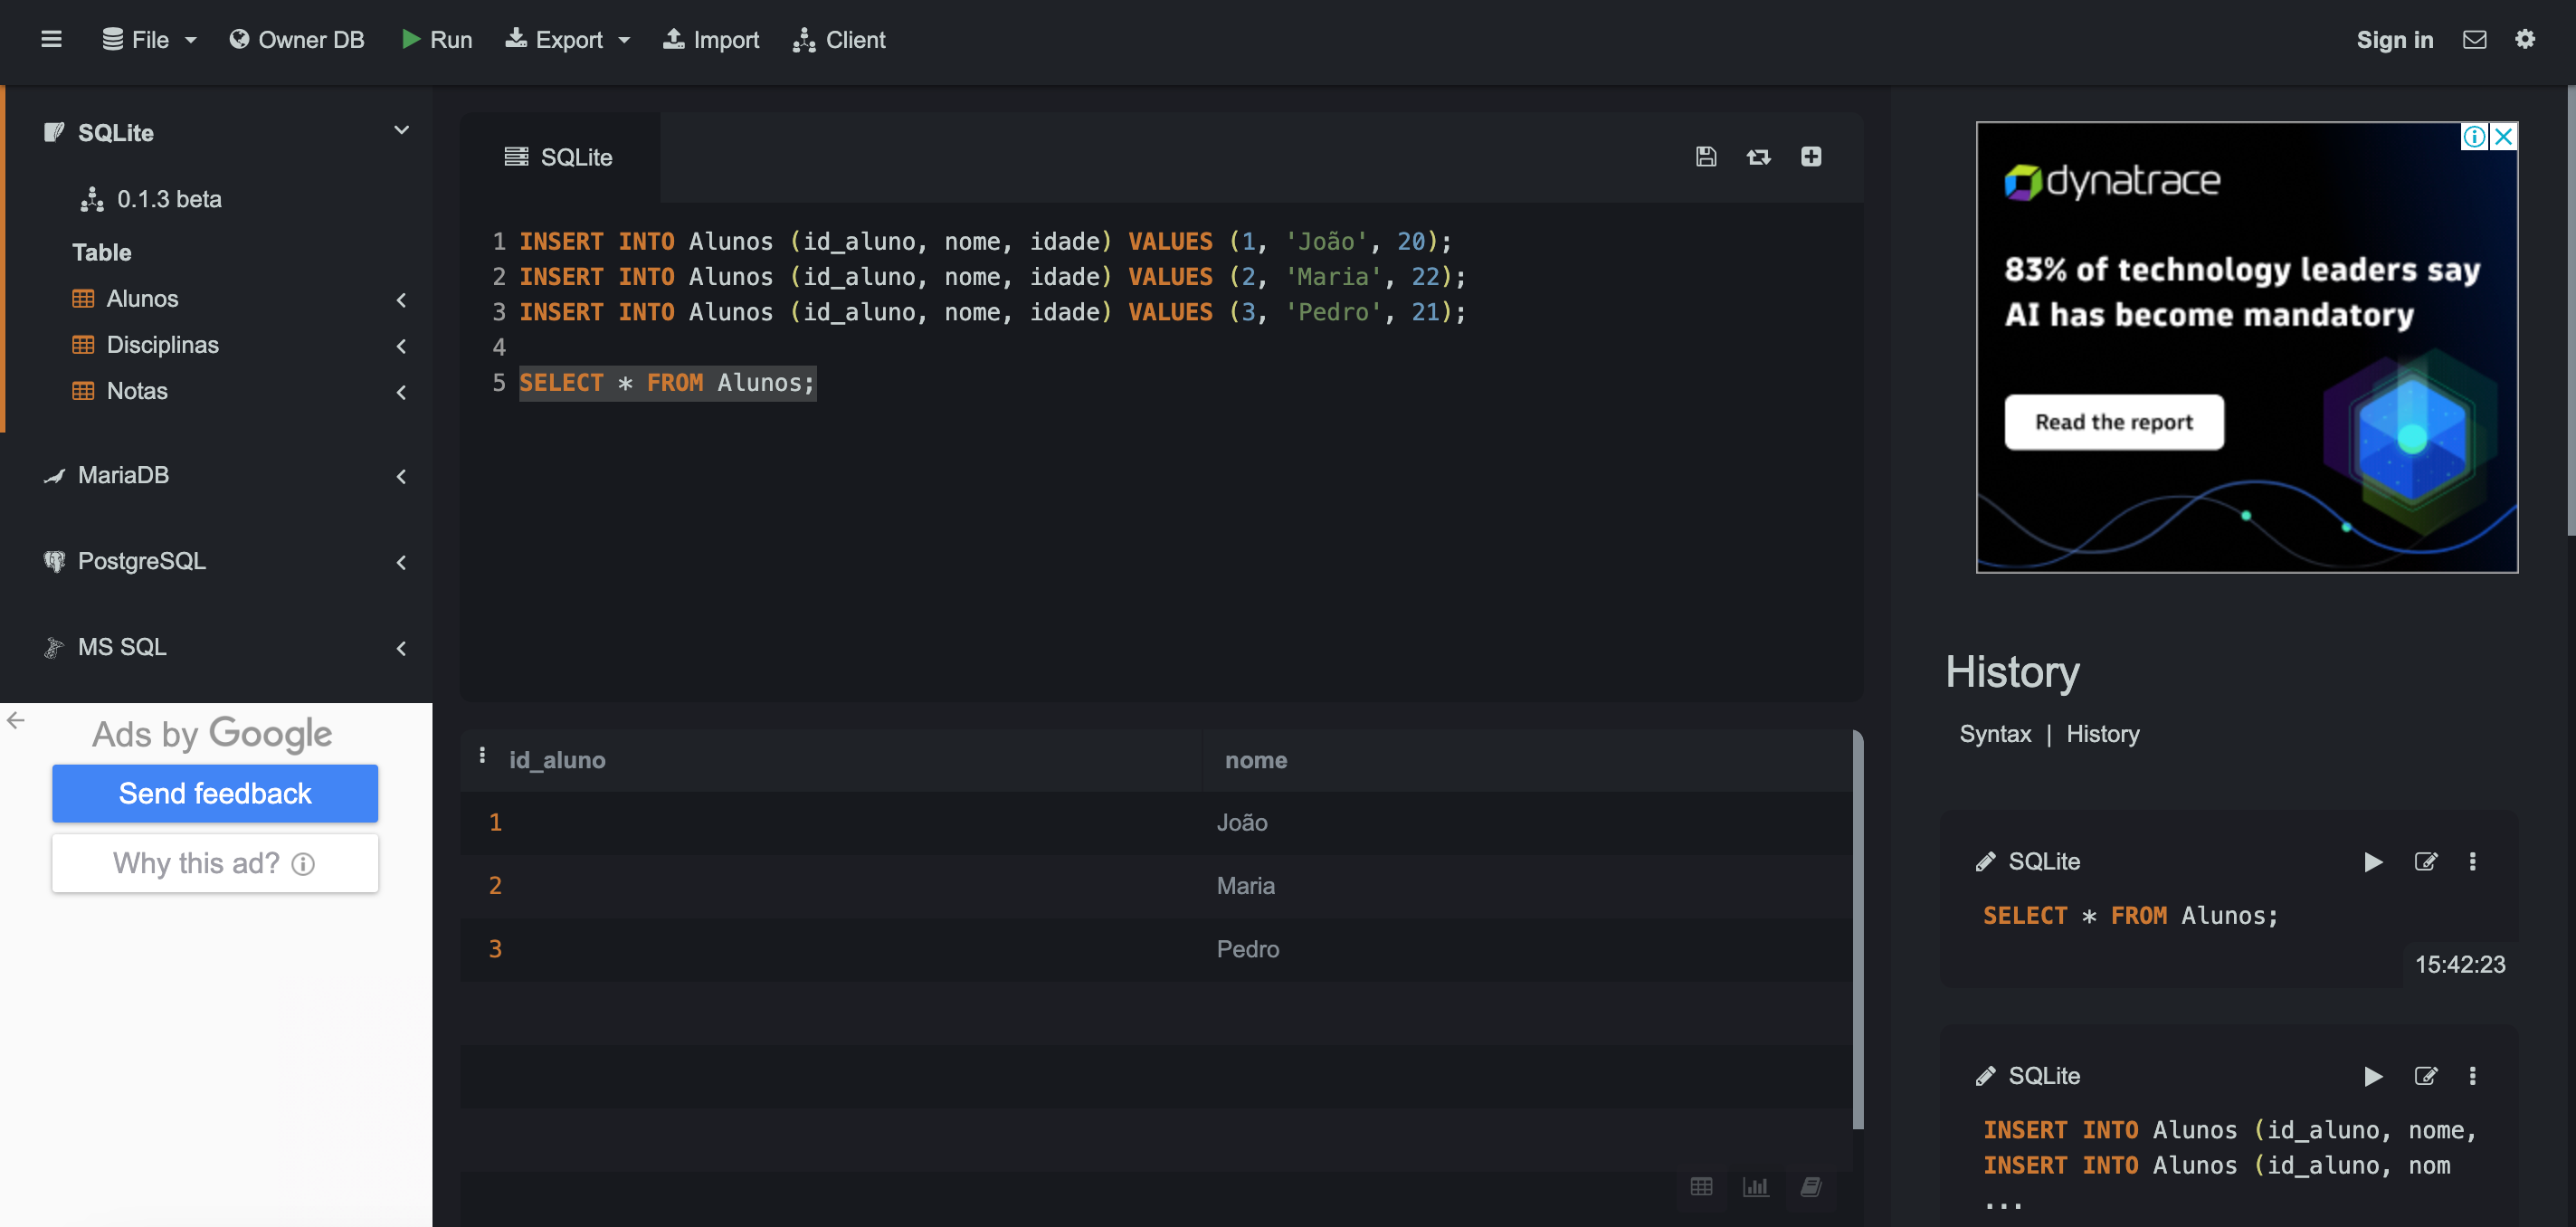
\includegraphics{insert_alunos.png}

\begin{itemize}
\tightlist
\item
  Passo 3: Inserir dados na tabela Disciplina.
\end{itemize}

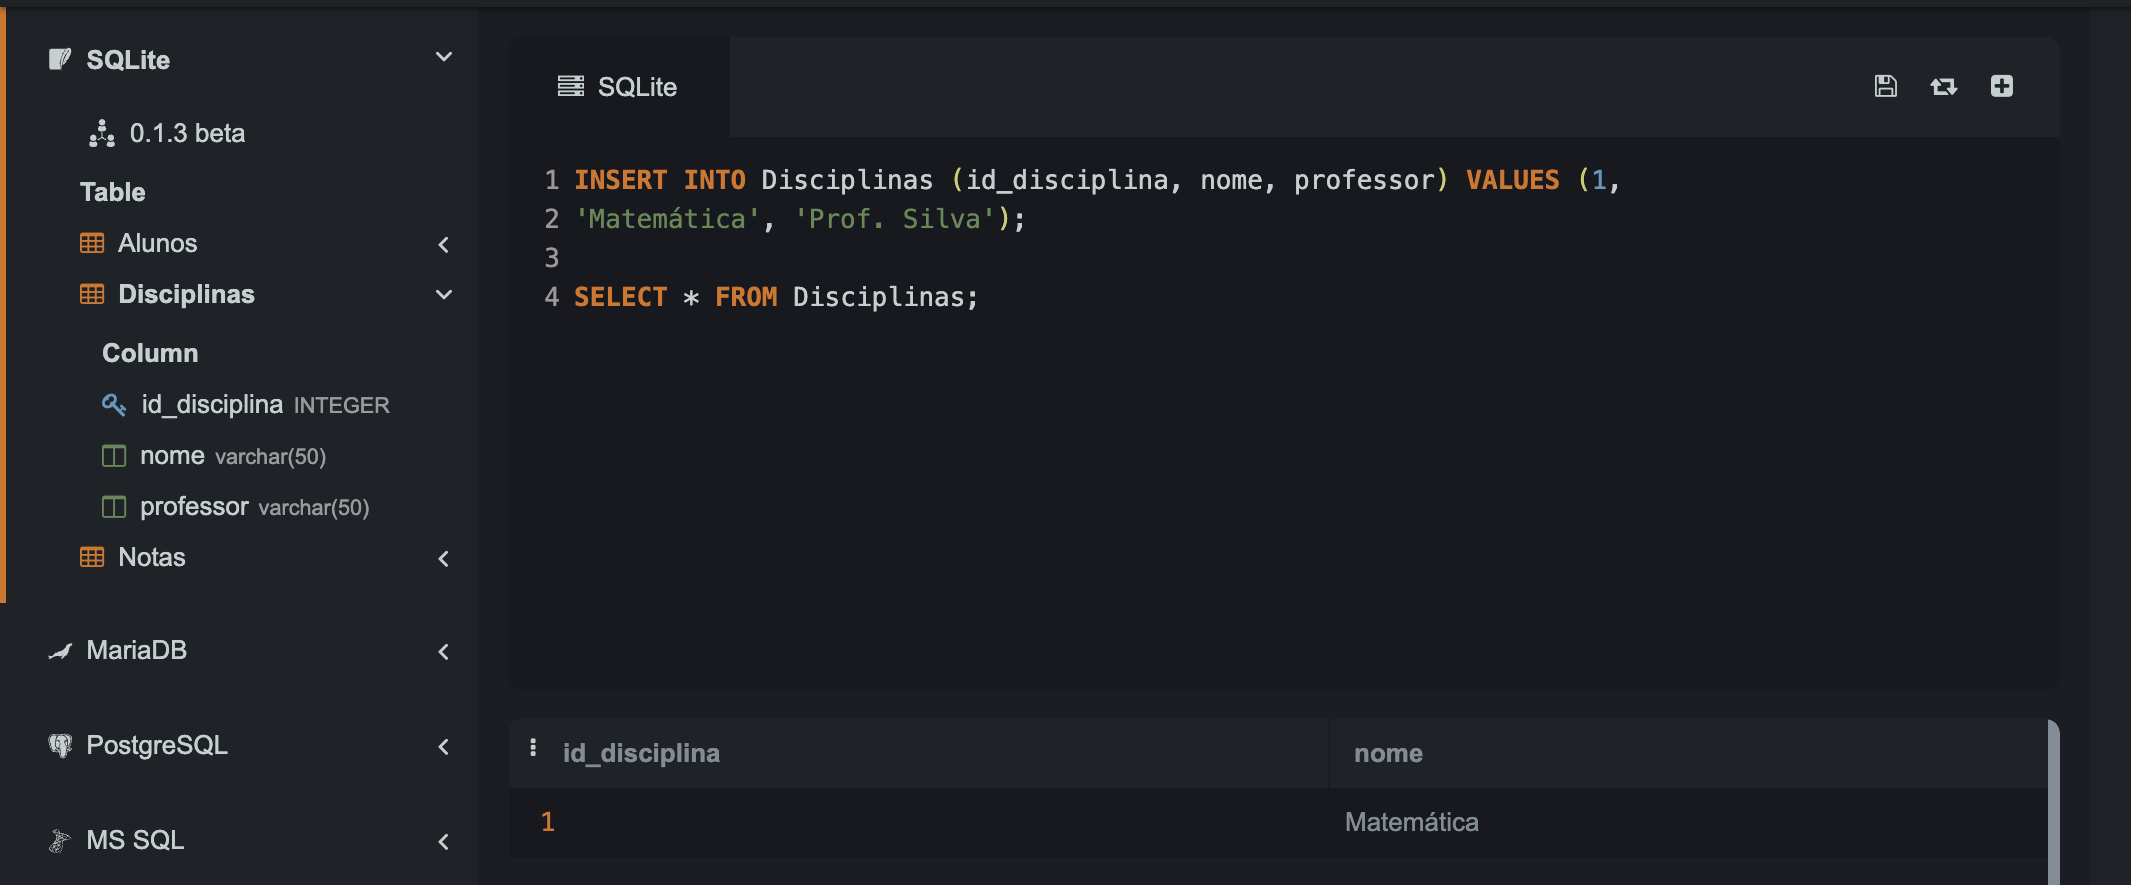
\includegraphics{insert_disciplina.png}

\begin{itemize}
\tightlist
\item
  Passo 4: Inserir dados na tabela Notas.
\end{itemize}

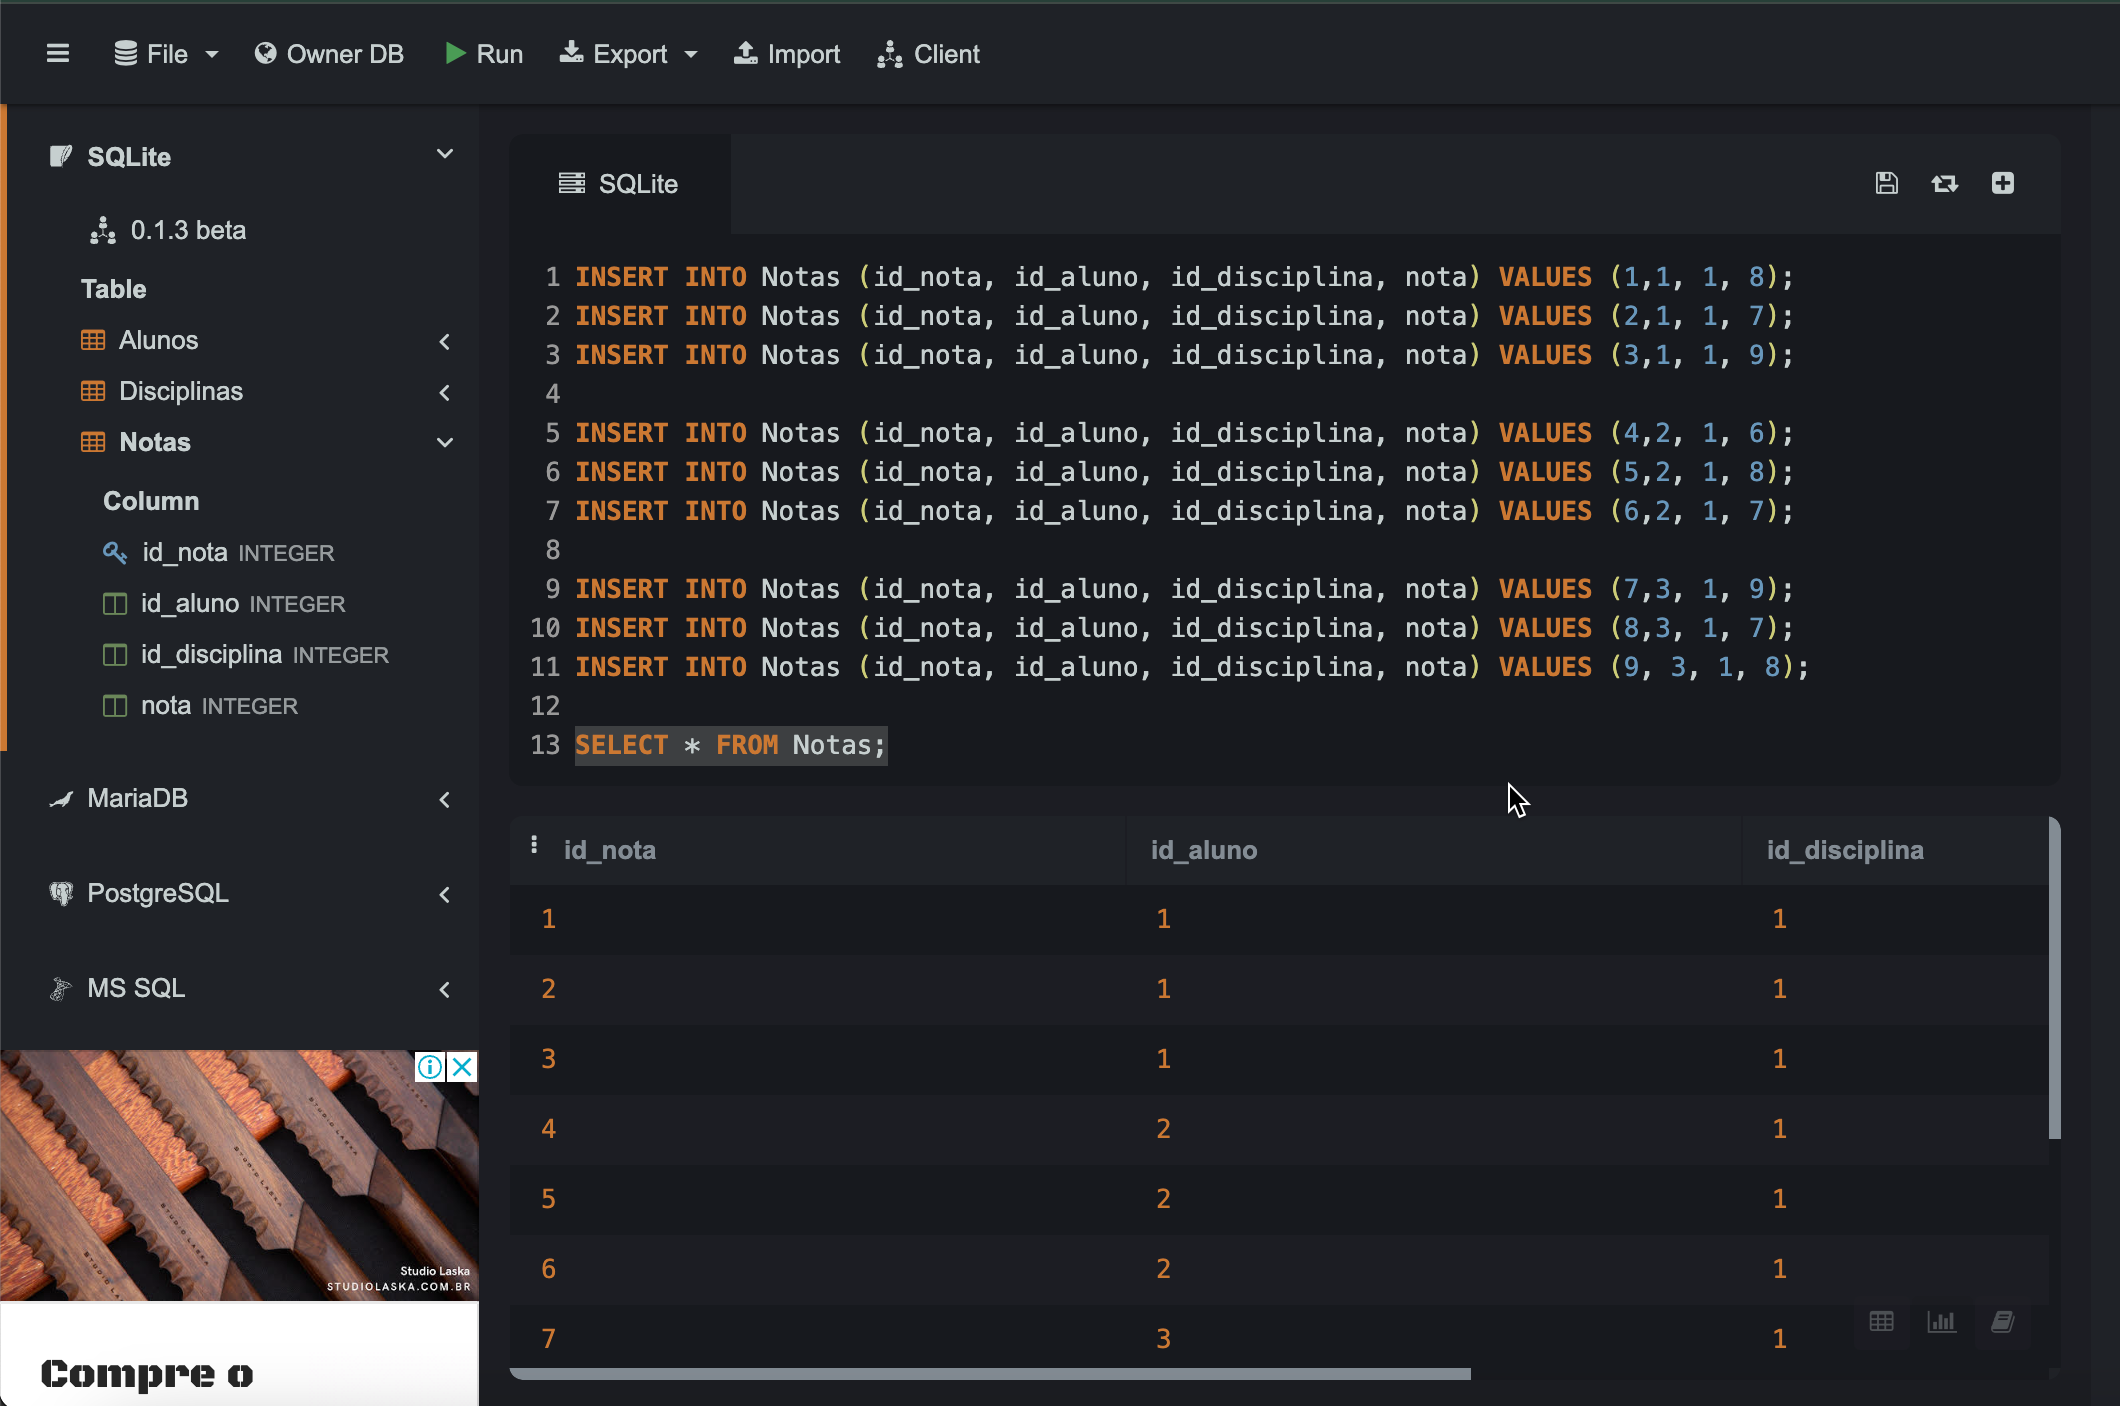
\includegraphics{insert_notas.png}

\begin{itemize}
\tightlist
\item
  Passo 5: Update de dados na tabela Alunos.
\end{itemize}

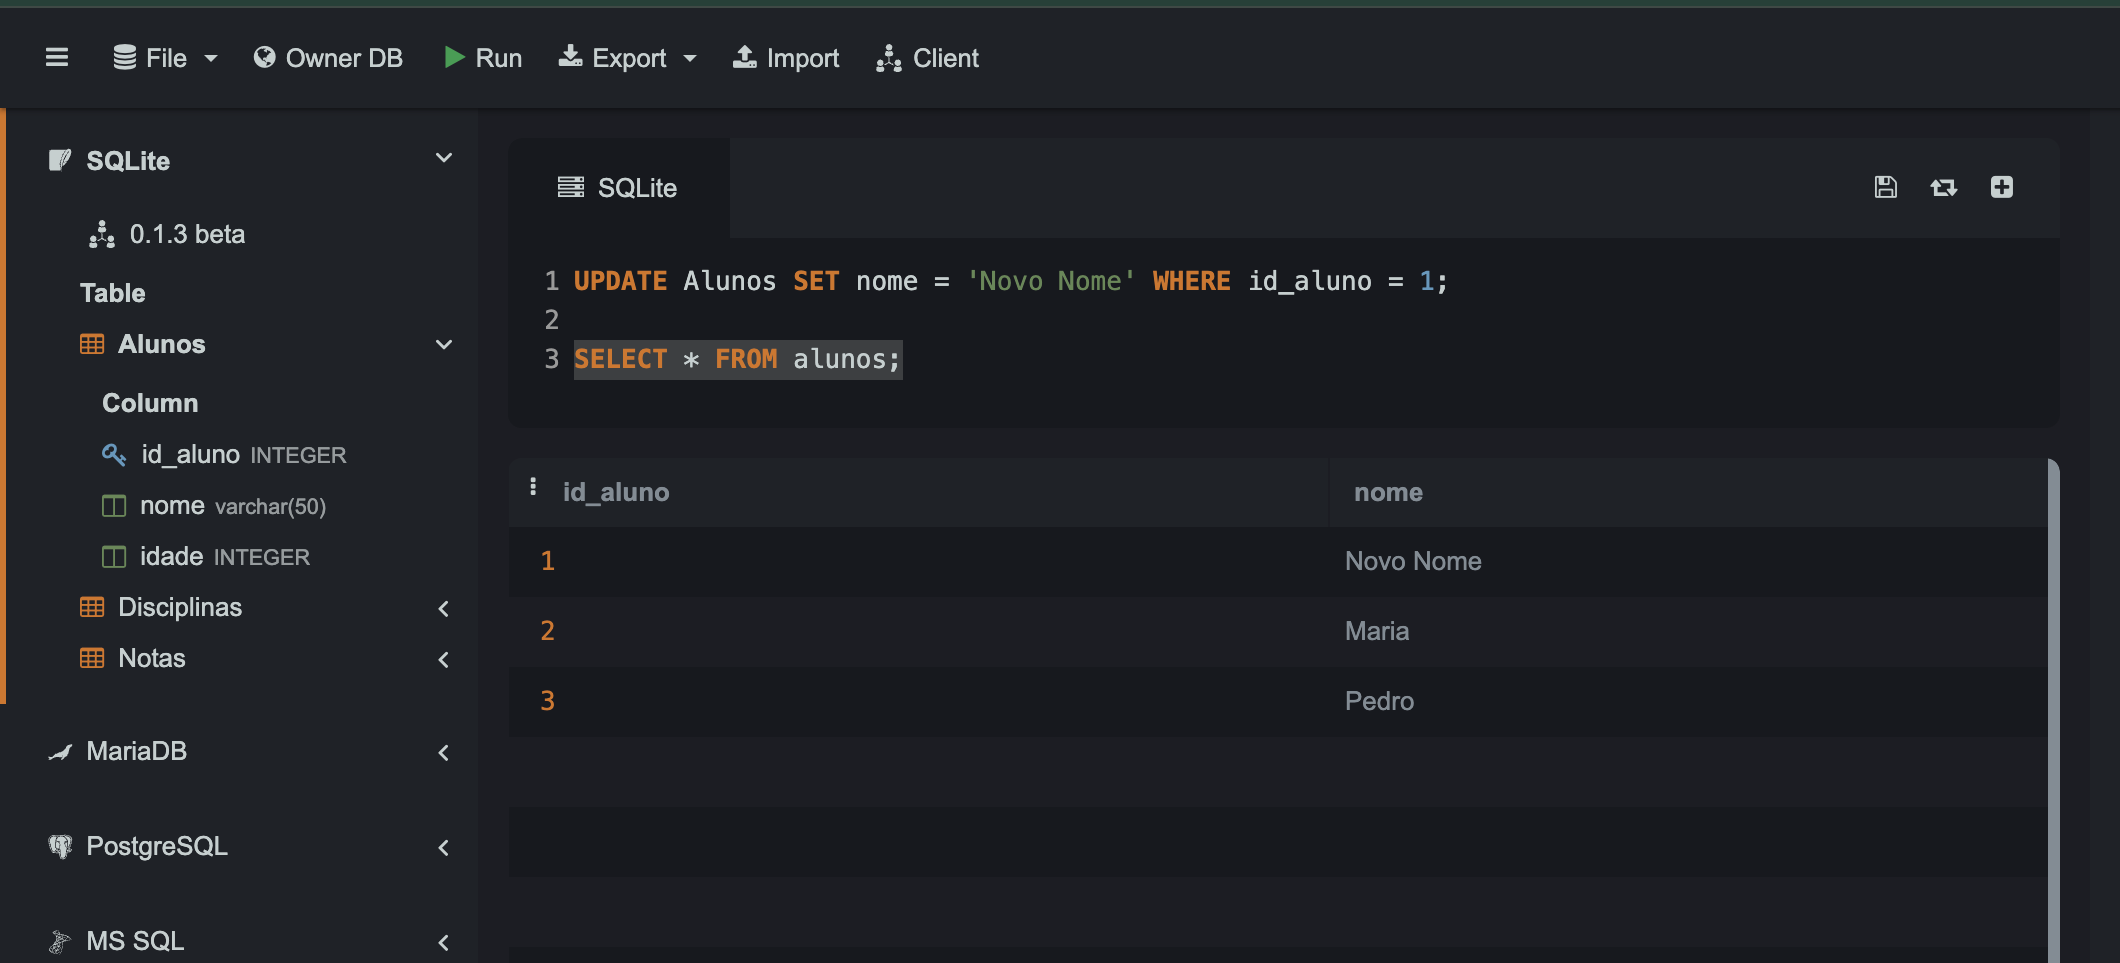
\includegraphics{update_alunos.png}

\begin{itemize}
\tightlist
\item
  Passo 6: Visualizando as tabelas interligadas.
\end{itemize}

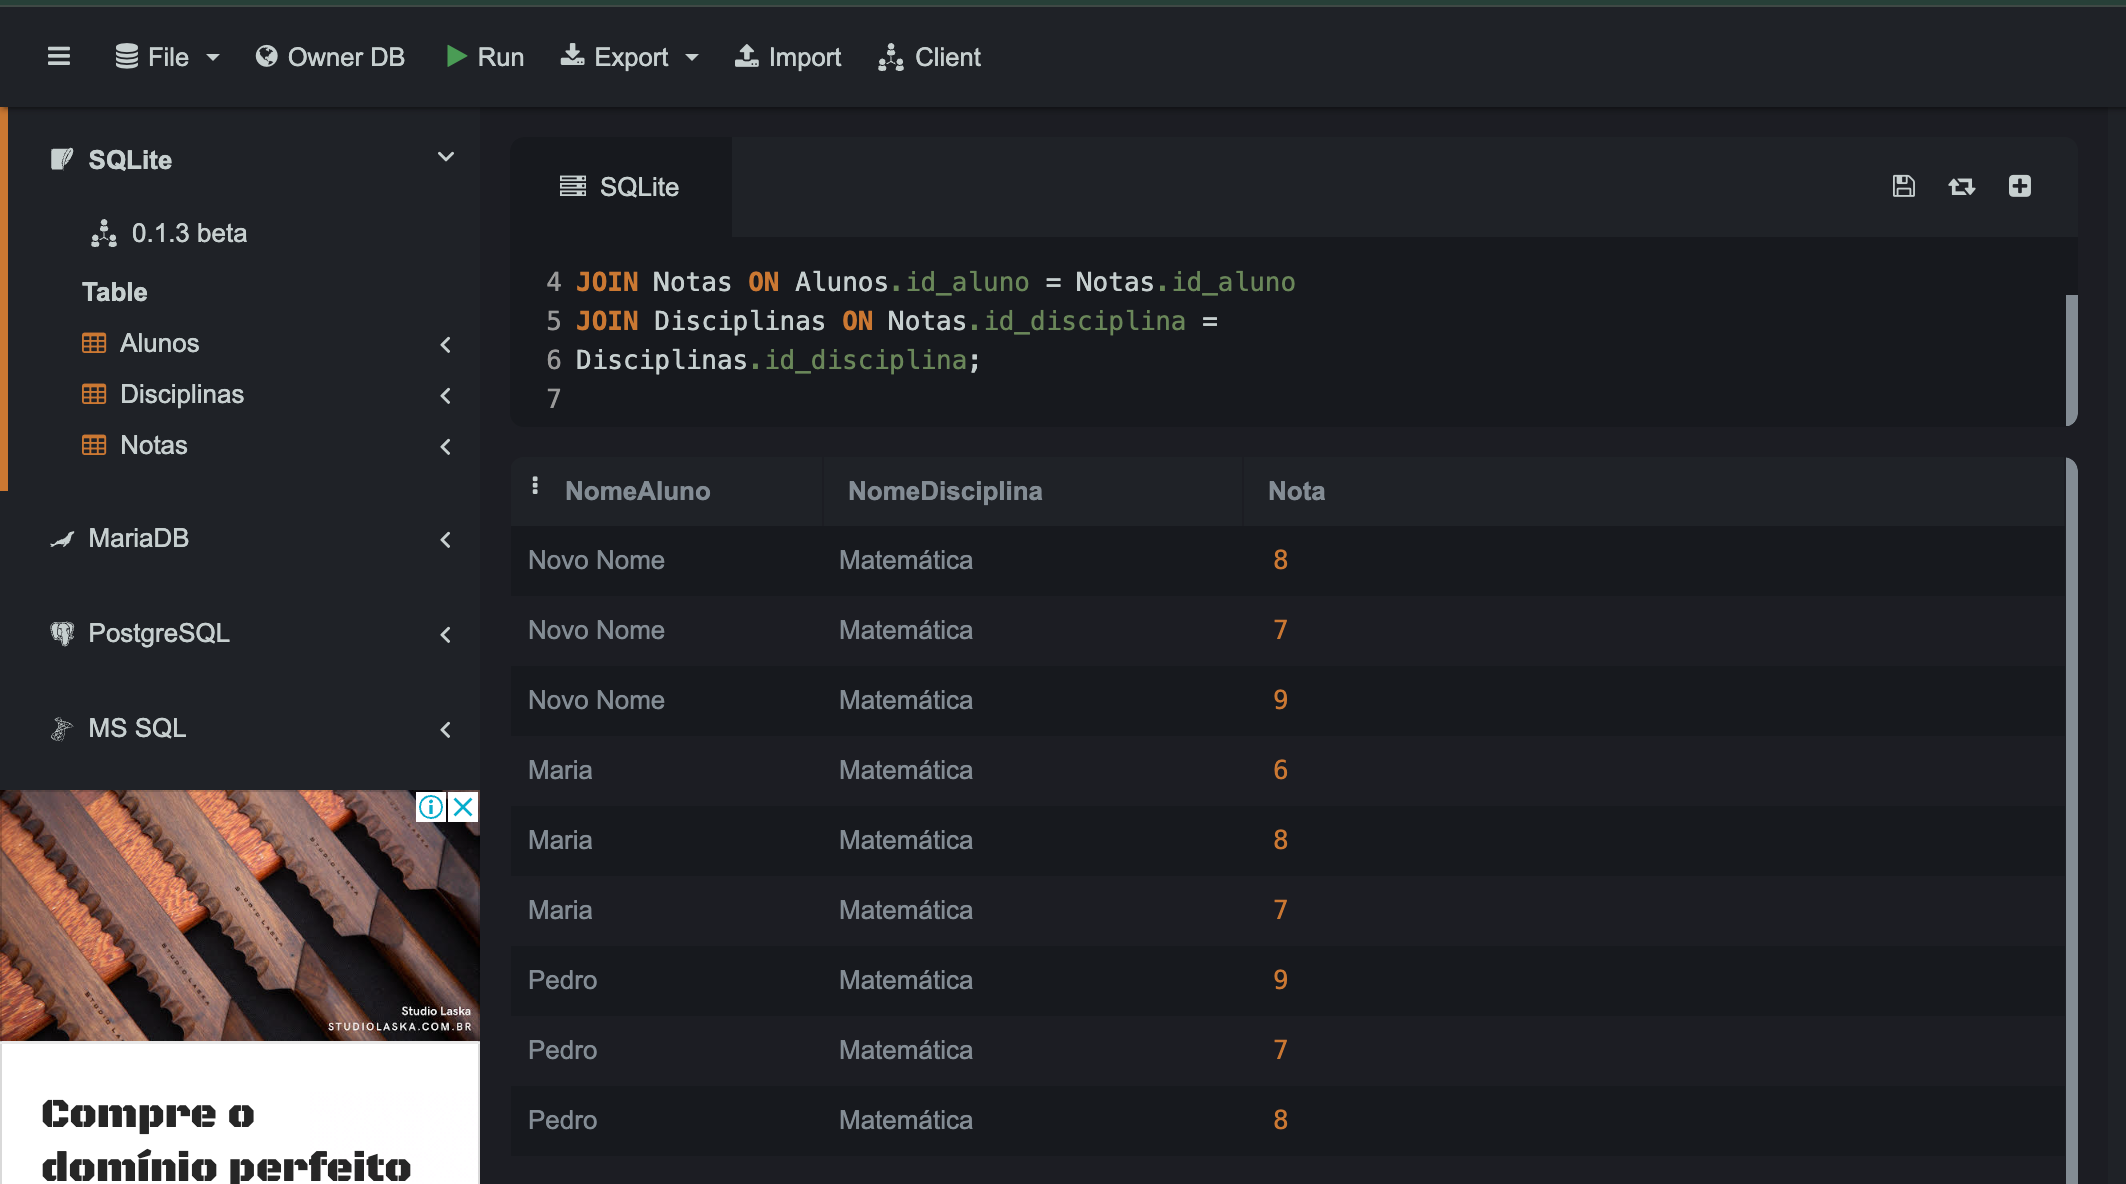
\includegraphics{visualizar.png}

\emph{Questão 2. Na ferramenta SQLite IDE, insira linhas em todas as
tabelas do BD criado.}

\subsubsection{Solução:}\label{soluuxe7uxe3o-1}

\begin{itemize}
\tightlist
\item
  Passo 1: Insert na tabela Alunos.
\end{itemize}

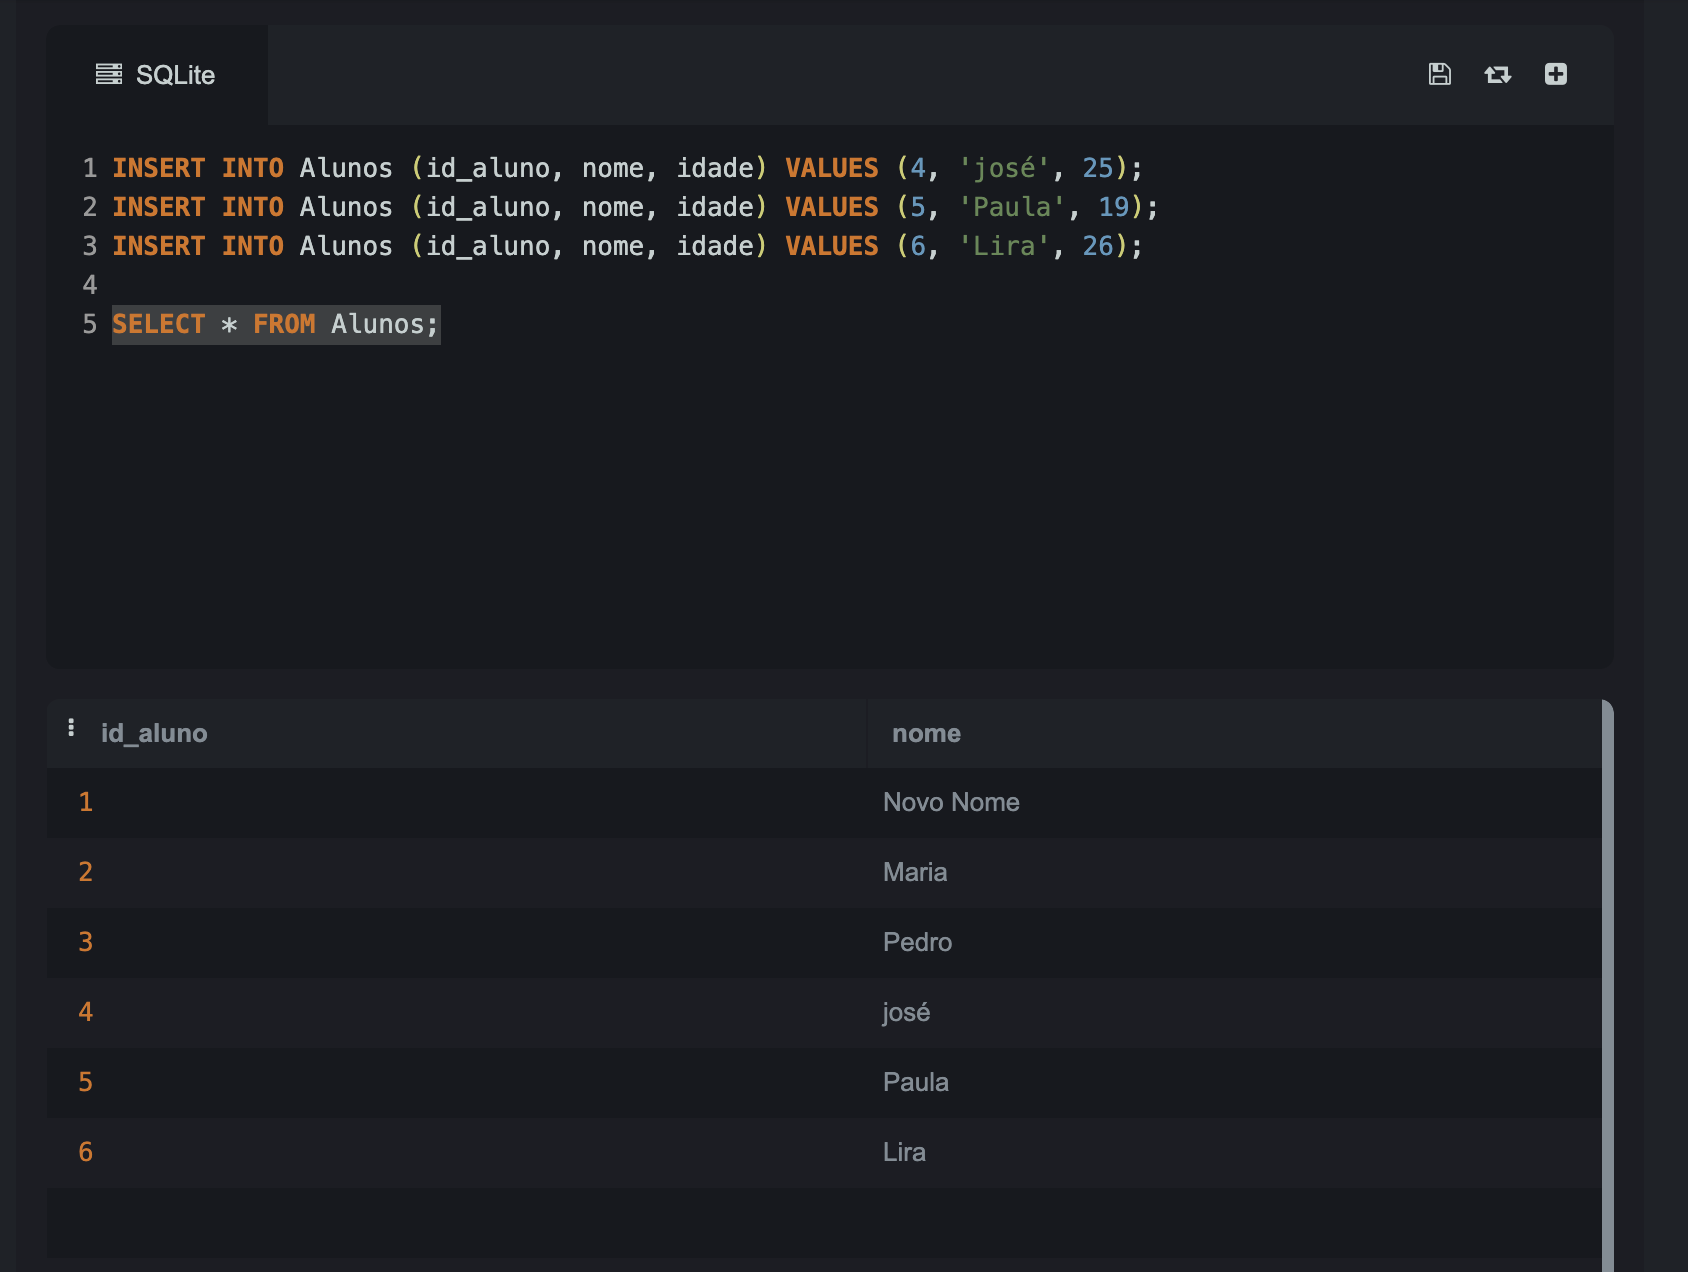
\includegraphics{insert_2_alunos.png}

\begin{itemize}
\tightlist
\item
  Passo 2: Insert na tabela Disciplinas.
\end{itemize}

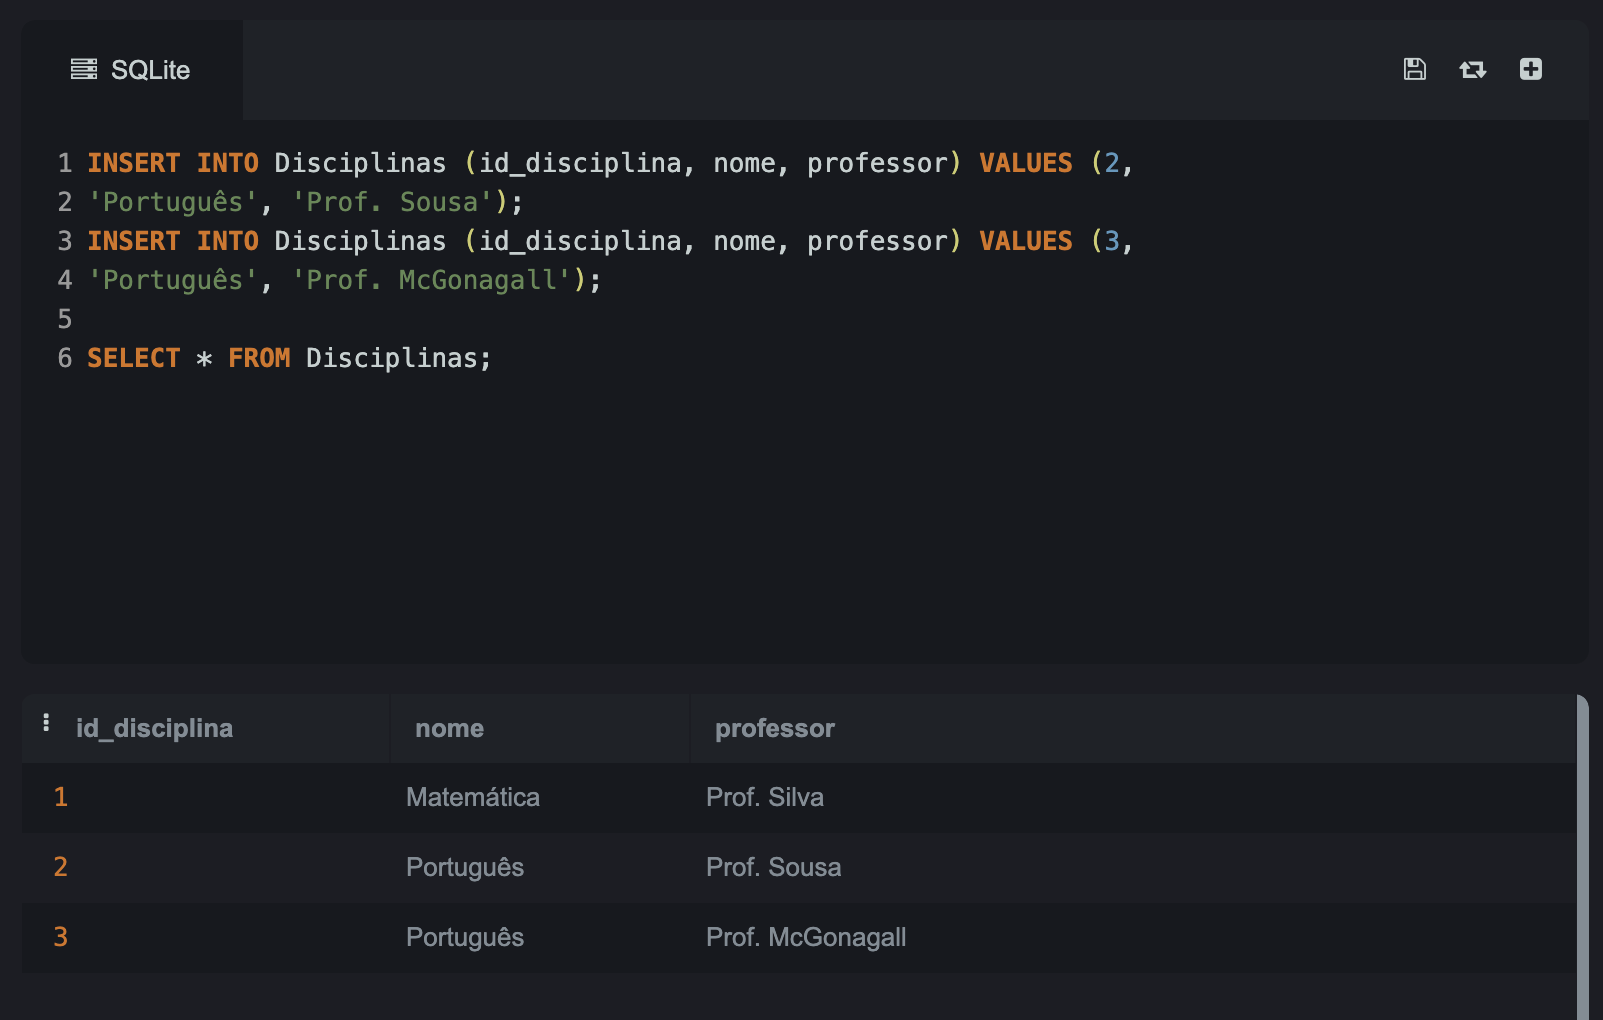
\includegraphics{insert_2_disciplinas.png}

\begin{itemize}
\tightlist
\item
  Passo 3: Insert na tabela Notas.
\end{itemize}

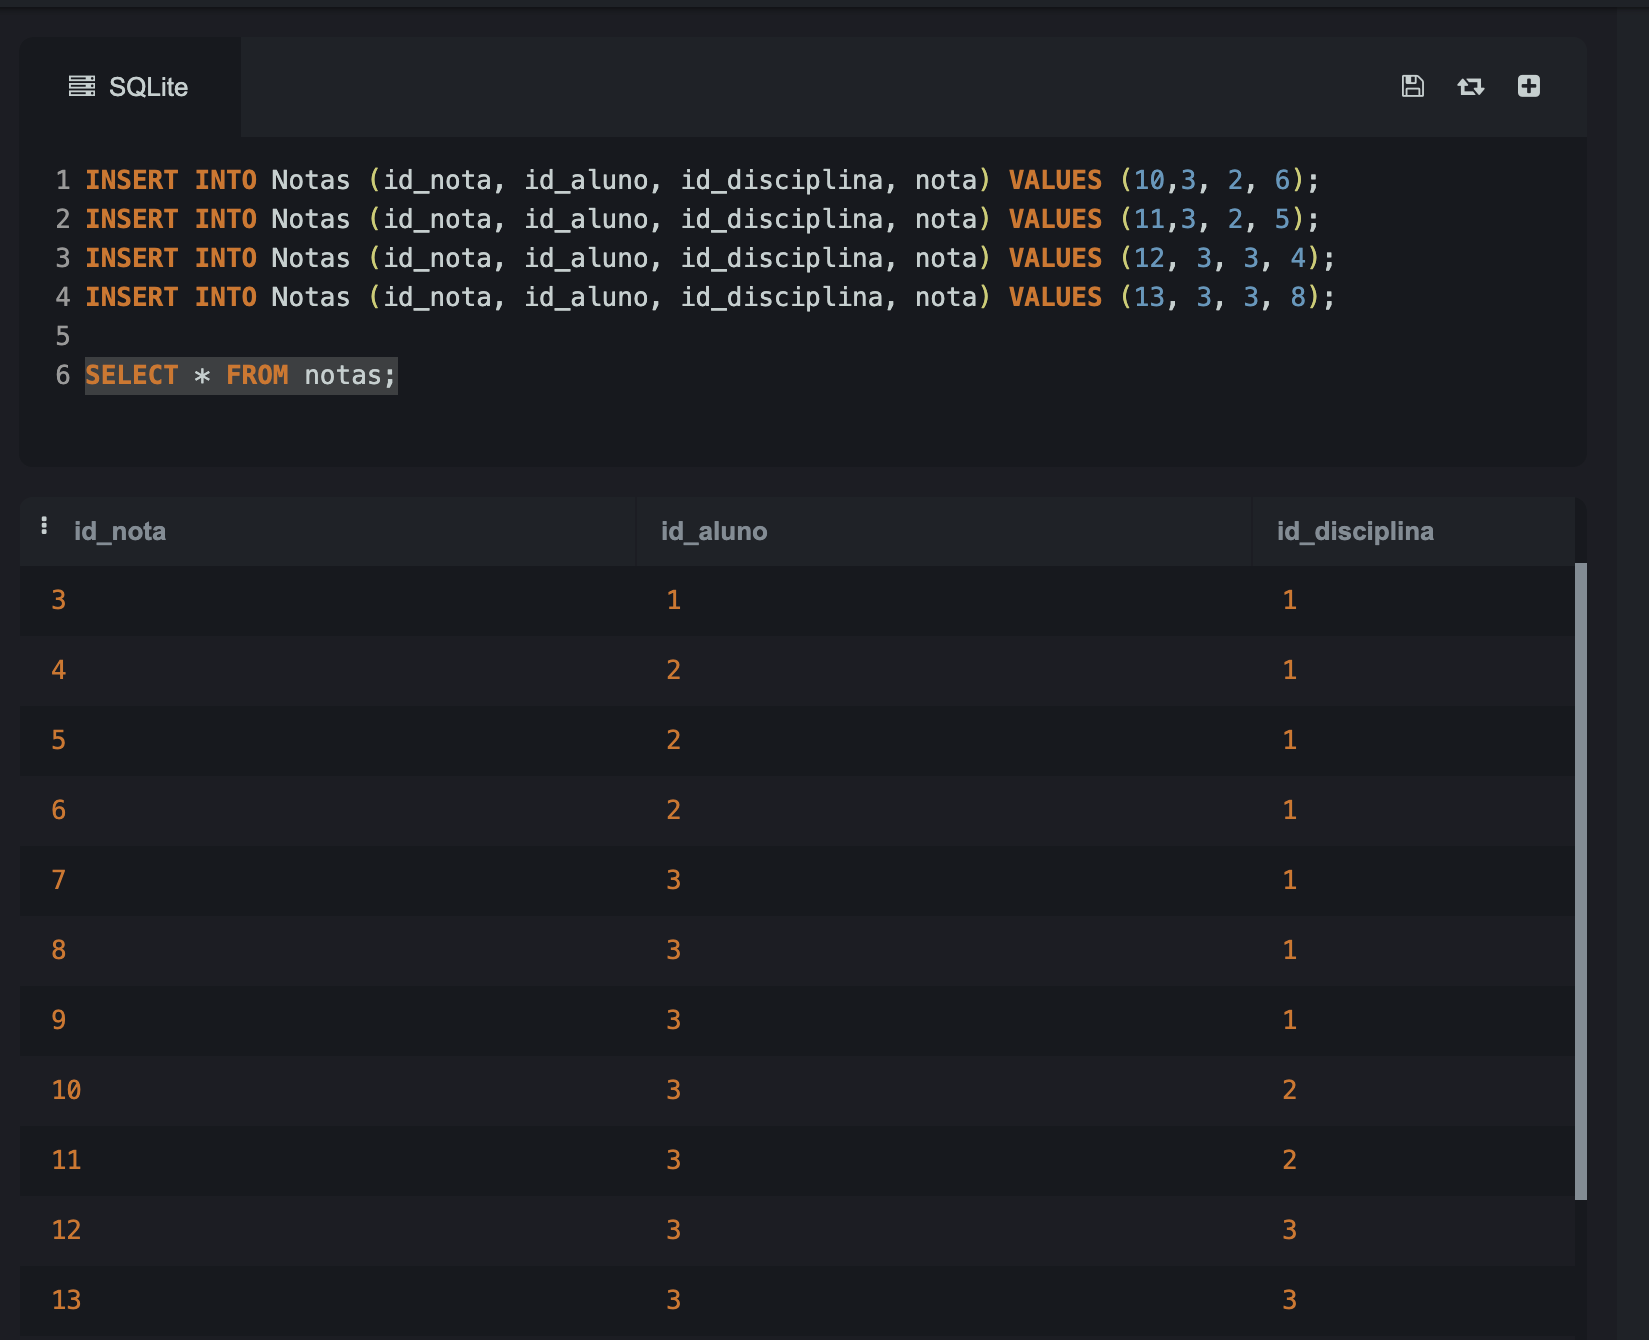
\includegraphics{insert_2_notas.png}

\begin{itemize}
\tightlist
\item
  Passo 3: Insert na tabela Alunos.
\end{itemize}

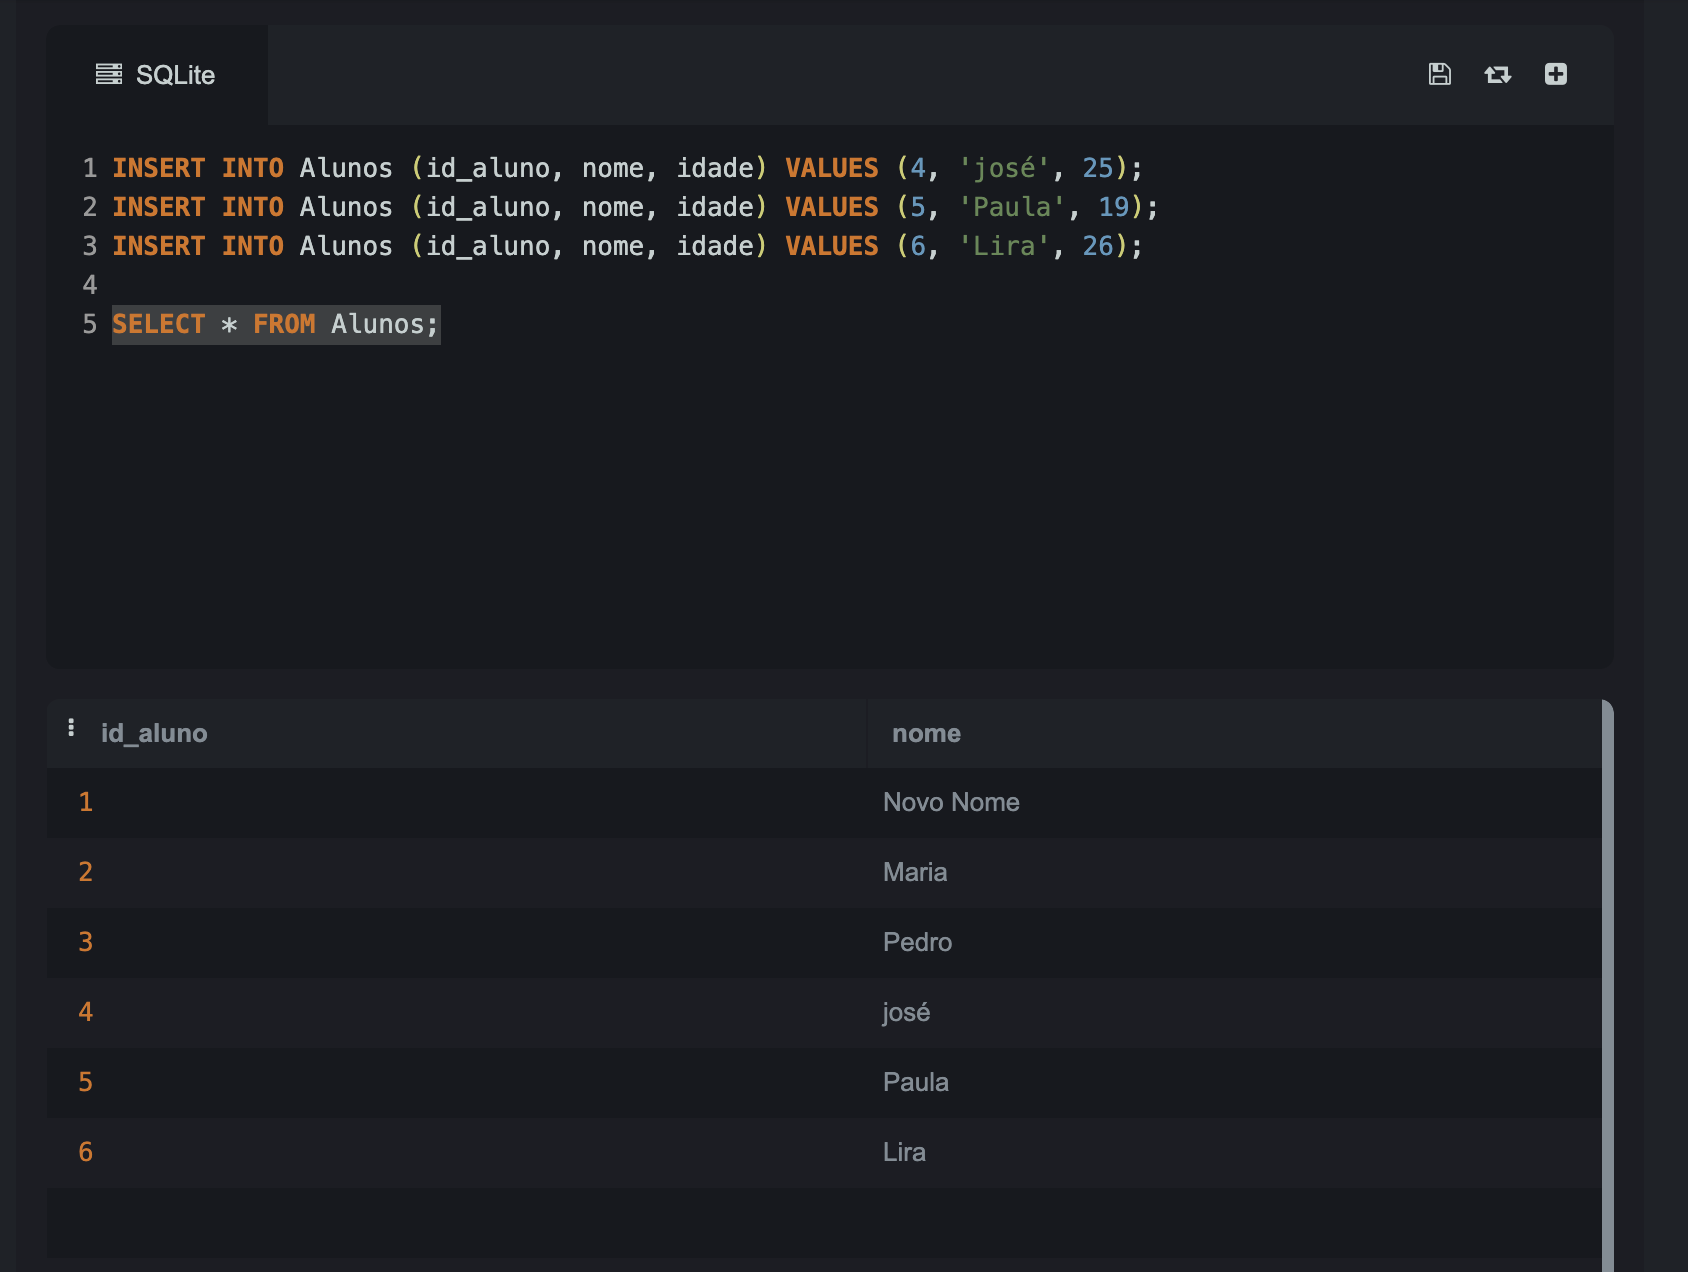
\includegraphics{insert_2_alunos.png}

\emph{Questão 3. Na ferramenta SQLite, gere o BD na forma de um arquivo
e armazene-o em uma pasta/diretório no seu computador.}

\subsubsection{Solução:}\label{soluuxe7uxe3o-2}

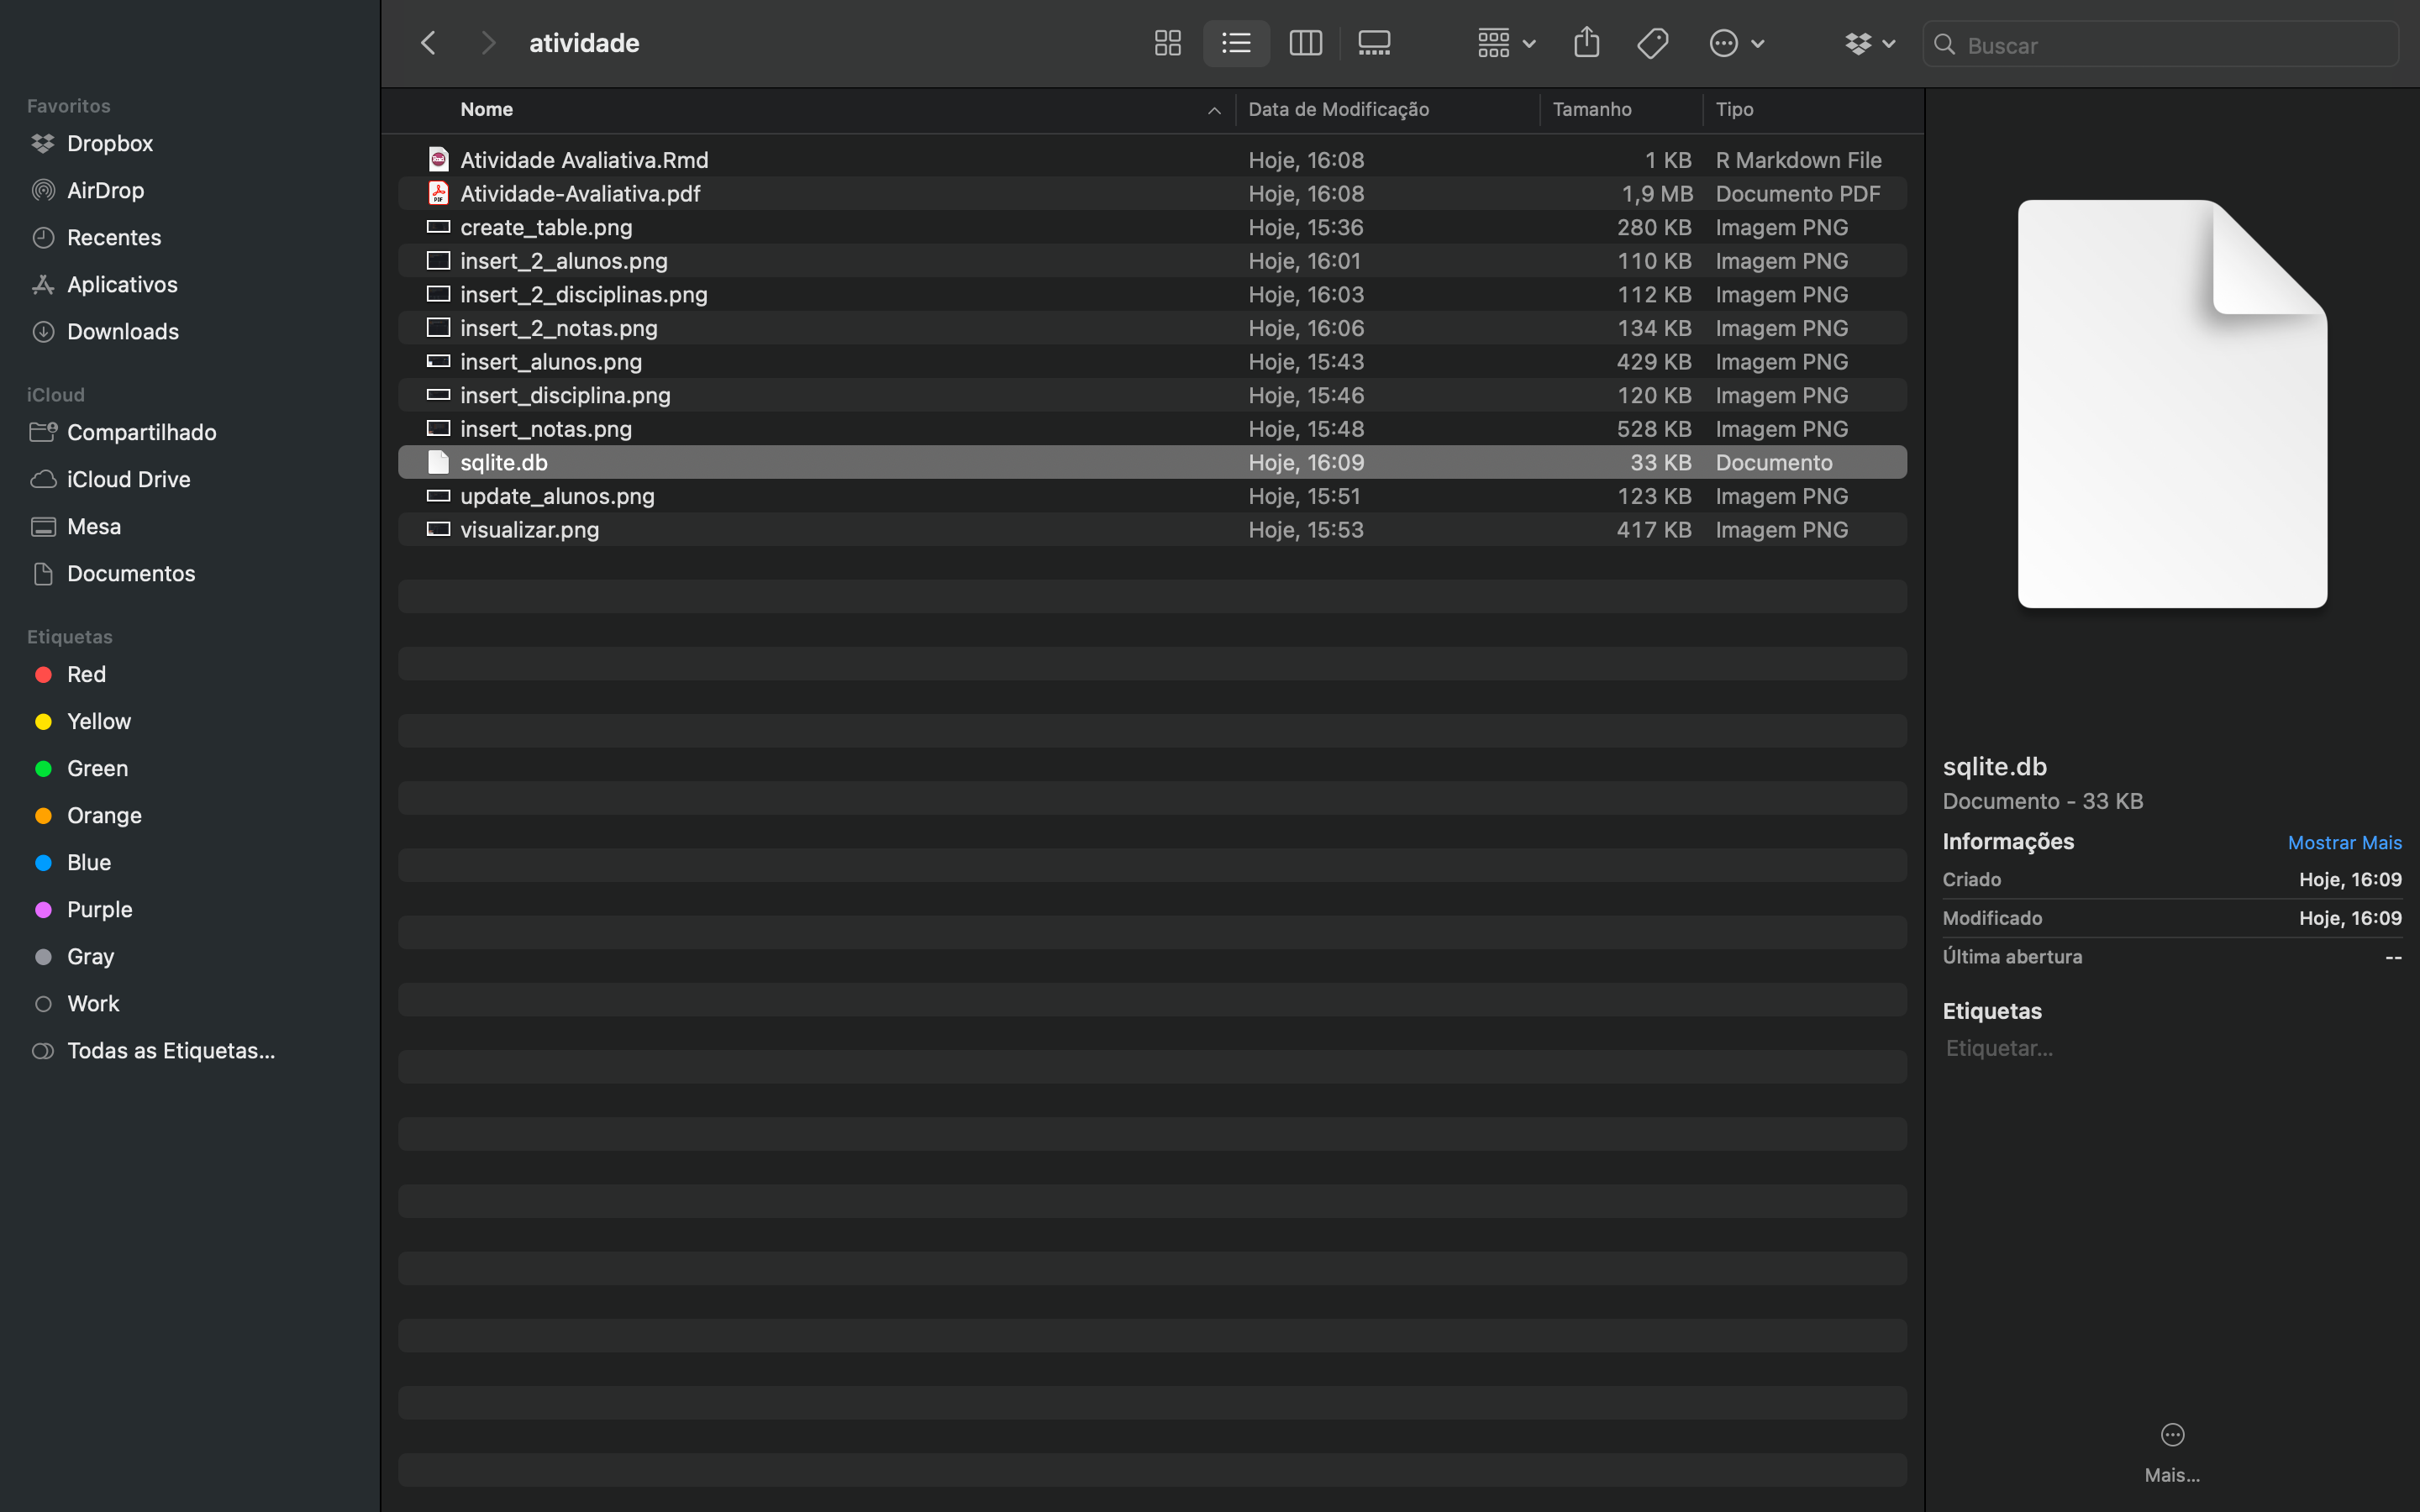
\includegraphics{bd.png}

\emph{Questão 4. No R, faça a conexão com o BD usando o arquivo gerado
no enunciado 3.}

\subsubsection{Solução}\label{soluuxe7uxe3o-3}

\begin{Shaded}
\begin{Highlighting}[]
\FunctionTok{library}\NormalTok{(}\StringTok{"RSQLite"}\NormalTok{)}
\FunctionTok{setwd}\NormalTok{(}\StringTok{"/Users/anamaria/especializacao/modulo\_2/atividade/"}\NormalTok{)}
\NormalTok{conexao }\OtherTok{\textless{}{-}}\NormalTok{ RSQLite}\SpecialCharTok{::}\FunctionTok{dbConnect}\NormalTok{(RSQLite}\SpecialCharTok{::}\FunctionTok{SQLite}\NormalTok{(), }\AttributeTok{dbname =} \StringTok{"sqlite.db"}\NormalTok{)}
\end{Highlighting}
\end{Shaded}

\begin{Shaded}
\begin{Highlighting}[]
\NormalTok{DBI}\SpecialCharTok{::}\FunctionTok{dbListTables}\NormalTok{(conexao)}
\end{Highlighting}
\end{Shaded}

\begin{verbatim}
## [1] "Alunos"      "Disciplinas" "Notas"
\end{verbatim}

\emph{Questão 5. No R, construa três consultas SQL selecionando
diretamente do BD linhas das tabelas utilizando a cláusula WHERE.}

\subsubsection{Solução}\label{soluuxe7uxe3o-4}

\begin{Shaded}
\begin{Highlighting}[]
\CommentTok{{-}{-} Consulta na tabela Alunos}
\KeywordTok{SELECT} \OperatorTok{*} \KeywordTok{FROM}\NormalTok{ Alunos }\KeywordTok{where}\NormalTok{ nome }\OperatorTok{=}\StringTok{\textquotesingle{}Paula\textquotesingle{}}\NormalTok{;}
\end{Highlighting}
\end{Shaded}

\begin{longtable}[]{@{}rlr@{}}
\caption{1 records}\tabularnewline
\toprule\noalign{}
id\_aluno & nome & idade \\
\midrule\noalign{}
\endfirsthead
\toprule\noalign{}
id\_aluno & nome & idade \\
\midrule\noalign{}
\endhead
\bottomrule\noalign{}
\endlastfoot
5 & Paula & 19 \\
\end{longtable}

\begin{Shaded}
\begin{Highlighting}[]
\CommentTok{{-}{-} Consulta na tabela Disciplina}
\KeywordTok{SELECT} \OperatorTok{*} \KeywordTok{FROM}\NormalTok{ Disciplinas }\KeywordTok{where}\NormalTok{ nome }\OperatorTok{=}\StringTok{\textquotesingle{}Português\textquotesingle{}}\NormalTok{;}
\end{Highlighting}
\end{Shaded}

\begin{longtable}[]{@{}lll@{}}
\caption{2 records}\tabularnewline
\toprule\noalign{}
id\_disciplina & nome & professor \\
\midrule\noalign{}
\endfirsthead
\toprule\noalign{}
id\_disciplina & nome & professor \\
\midrule\noalign{}
\endhead
\bottomrule\noalign{}
\endlastfoot
2 & Português & Prof.~Sousa \\
3 & Português & Prof.~McGonagall \\
\end{longtable}

\begin{Shaded}
\begin{Highlighting}[]
\CommentTok{{-}{-} Consulta na tabela Disciplina}
\KeywordTok{SELECT} \OperatorTok{*} \KeywordTok{FROM}\NormalTok{ Notas }\KeywordTok{where}\NormalTok{ nota }\OperatorTok{\textgreater{}} \DecValTok{8}\NormalTok{;}
\end{Highlighting}
\end{Shaded}

\begin{longtable}[]{@{}rrrr@{}}
\caption{2 records}\tabularnewline
\toprule\noalign{}
id\_nota & id\_aluno & id\_disciplina & nota \\
\midrule\noalign{}
\endfirsthead
\toprule\noalign{}
id\_nota & id\_aluno & id\_disciplina & nota \\
\midrule\noalign{}
\endhead
\bottomrule\noalign{}
\endlastfoot
3 & 1 & 1 & 9 \\
7 & 3 & 1 & 9 \\
\end{longtable}

\emph{Questão 6. No R, faça a importação das tabelas para data frames.}

\subsubsection{Solução}\label{soluuxe7uxe3o-5}

\begin{itemize}
\tightlist
\item
  Dataframe Alunos:
\end{itemize}

\begin{Shaded}
\begin{Highlighting}[]
\FunctionTok{library}\NormalTok{(}\StringTok{"dplyr"}\NormalTok{)}
\end{Highlighting}
\end{Shaded}

\begin{verbatim}
## 
## Attaching package: 'dplyr'
\end{verbatim}

\begin{verbatim}
## The following objects are masked from 'package:stats':
## 
##     filter, lag
\end{verbatim}

\begin{verbatim}
## The following objects are masked from 'package:base':
## 
##     intersect, setdiff, setequal, union
\end{verbatim}

\begin{Shaded}
\begin{Highlighting}[]
\FunctionTok{library}\NormalTok{(}\StringTok{"tibble"}\NormalTok{)}
\NormalTok{alunos\_tbl }\OtherTok{\textless{}{-}}\NormalTok{ dplyr}\SpecialCharTok{::}\FunctionTok{tbl}\NormalTok{(conexao,}\StringTok{"Alunos"}\NormalTok{)}
\NormalTok{alunos\_df }\OtherTok{\textless{}{-}}\NormalTok{ dplyr}\SpecialCharTok{::}\FunctionTok{collect}\NormalTok{(alunos\_tbl)}
\end{Highlighting}
\end{Shaded}

\begin{Shaded}
\begin{Highlighting}[]
\NormalTok{alunos\_df}
\end{Highlighting}
\end{Shaded}

\begin{verbatim}
## # A tibble: 6 x 3
##   id_aluno nome      idade
##      <int> <chr>     <int>
## 1        1 Novo Nome    20
## 2        2 Maria        22
## 3        3 Pedro        21
## 4        4 josé         25
## 5        5 Paula        19
## 6        6 Lira         26
\end{verbatim}

\begin{itemize}
\tightlist
\item
  Dataframe Disciplinas:
\end{itemize}

\begin{Shaded}
\begin{Highlighting}[]
\NormalTok{disciplinas\_tbl }\OtherTok{\textless{}{-}}\NormalTok{ dplyr}\SpecialCharTok{::}\FunctionTok{tbl}\NormalTok{(conexao,}\StringTok{"Disciplinas"}\NormalTok{)}
\NormalTok{disciplinas\_df }\OtherTok{\textless{}{-}}\NormalTok{ dplyr}\SpecialCharTok{::}\FunctionTok{collect}\NormalTok{(disciplinas\_tbl)}
\end{Highlighting}
\end{Shaded}

\begin{Shaded}
\begin{Highlighting}[]
\NormalTok{disciplinas\_df}
\end{Highlighting}
\end{Shaded}

\begin{verbatim}
## # A tibble: 3 x 3
##   id_disciplina nome       professor       
##           <int> <chr>      <chr>           
## 1             1 Matemática Prof. Silva     
## 2             2 Português  Prof. Sousa     
## 3             3 Português  Prof. McGonagall
\end{verbatim}

\begin{itemize}
\tightlist
\item
  Dataframe Notas:
\end{itemize}

\begin{Shaded}
\begin{Highlighting}[]
\NormalTok{notas\_tbl }\OtherTok{\textless{}{-}}\NormalTok{ dplyr}\SpecialCharTok{::}\FunctionTok{tbl}\NormalTok{(conexao,}\StringTok{"Notas"}\NormalTok{)}
\NormalTok{notas\_df }\OtherTok{\textless{}{-}}\NormalTok{ dplyr}\SpecialCharTok{::}\FunctionTok{collect}\NormalTok{(notas\_tbl)}
\NormalTok{notas\_df}
\end{Highlighting}
\end{Shaded}

\begin{verbatim}
## # A tibble: 13 x 4
##    id_nota id_aluno id_disciplina  nota
##      <int>    <int>         <int> <int>
##  1       1        1             1     8
##  2       2        1             1     7
##  3       3        1             1     9
##  4       4        2             1     6
##  5       5        2             1     8
##  6       6        2             1     7
##  7       7        3             1     9
##  8       8        3             1     7
##  9       9        3             1     8
## 10      10        3             2     6
## 11      11        3             2     5
## 12      12        3             3     4
## 13      13        3             3     8
\end{verbatim}

\emph{Questõ 7. No R, faça consultas utilizando select() do pacote dplyr
nos objetos tibble correspondentes aos data frames gerados no enunciado
6.}

\subsubsection{Solução}\label{soluuxe7uxe3o-6}

\begin{Shaded}
\begin{Highlighting}[]
\NormalTok{alunos1 }\OtherTok{\textless{}{-}}\NormalTok{ dplyr}\SpecialCharTok{::}\FunctionTok{sql}\NormalTok{(}\StringTok{"SELECT * FROM Alunos WHERE idade \textgreater{} 22"}\NormalTok{)}
\NormalTok{alunos\_select }\OtherTok{\textless{}{-}}\NormalTok{ dplyr}\SpecialCharTok{::}\FunctionTok{tbl}\NormalTok{(conexao, alunos1)}
\NormalTok{alunos\_db\_select }\OtherTok{\textless{}{-}}\NormalTok{ dplyr}\SpecialCharTok{::}\FunctionTok{collect}\NormalTok{(alunos\_select)}
\NormalTok{alunos\_db\_select}
\end{Highlighting}
\end{Shaded}

\begin{verbatim}
## # A tibble: 2 x 3
##   id_aluno nome  idade
##      <int> <chr> <int>
## 1        4 josé     25
## 2        6 Lira     26
\end{verbatim}

\begin{Shaded}
\begin{Highlighting}[]
\NormalTok{disciplinas1 }\OtherTok{\textless{}{-}}\NormalTok{ dplyr}\SpecialCharTok{::}\FunctionTok{sql}\NormalTok{(}\StringTok{"SELECT * FROM Disciplinas WHERE nome != \textquotesingle{}Português\textquotesingle{}"}\NormalTok{)}
\NormalTok{disciplinas\_select }\OtherTok{\textless{}{-}}\NormalTok{ dplyr}\SpecialCharTok{::}\FunctionTok{tbl}\NormalTok{(conexao, disciplinas1)}
\NormalTok{disciplinas\_db\_select }\OtherTok{\textless{}{-}}\NormalTok{ dplyr}\SpecialCharTok{::}\FunctionTok{collect}\NormalTok{(disciplinas\_select)}
\NormalTok{disciplinas\_db\_select}
\end{Highlighting}
\end{Shaded}

\begin{verbatim}
## # A tibble: 1 x 3
##   id_disciplina nome       professor  
##           <int> <chr>      <chr>      
## 1             1 Matemática Prof. Silva
\end{verbatim}

\begin{Shaded}
\begin{Highlighting}[]
\NormalTok{notas1 }\OtherTok{\textless{}{-}}\NormalTok{ dplyr}\SpecialCharTok{::}\FunctionTok{sql}\NormalTok{(}\StringTok{"SELECT * FROM Notas WHERE nota \textless{}= 6"}\NormalTok{)}
\NormalTok{notas\_select }\OtherTok{\textless{}{-}}\NormalTok{ dplyr}\SpecialCharTok{::}\FunctionTok{tbl}\NormalTok{(conexao, notas1)}
\NormalTok{notas\_db\_select }\OtherTok{\textless{}{-}}\NormalTok{ dplyr}\SpecialCharTok{::}\FunctionTok{collect}\NormalTok{(notas\_select)}
\NormalTok{notas\_db\_select}
\end{Highlighting}
\end{Shaded}

\begin{verbatim}
## # A tibble: 4 x 4
##   id_nota id_aluno id_disciplina  nota
##     <int>    <int>         <int> <int>
## 1       4        2             1     6
## 2      10        3             2     6
## 3      11        3             2     5
## 4      12        3             3     4
\end{verbatim}

\emph{8.(opcional) Realize o mesmo processo (enunciados 2 até 7) para o
BD ``Animais de uma Fazenda'', disponível em
\href{https://drive.google.com/file/d/1manYTl1tuIXJYyc0jsub7sGmrS4AuGgD/view?usp=drive_link}{google
drive} (páginas 22 a 25, apostila de SQllite).}

\subsubsection{Solução}\label{soluuxe7uxe3o-7}

Para questão de otimização do relatório, irei omitir os prints da
criação do BD. O BD estará anexado no arquivo compactado que está
anexado.

\begin{itemize}
\tightlist
\item
  Conectando no BD
\end{itemize}

\begin{Shaded}
\begin{Highlighting}[]
\NormalTok{conexao\_animal }\OtherTok{\textless{}{-}}\NormalTok{ RSQLite}\SpecialCharTok{::}\FunctionTok{dbConnect}\NormalTok{(RSQLite}\SpecialCharTok{::}\FunctionTok{SQLite}\NormalTok{(), }\AttributeTok{dbname =} \StringTok{"animal.db"}\NormalTok{)}
\end{Highlighting}
\end{Shaded}

\begin{itemize}
\tightlist
\item
  Realizar consultas utilizando a cláusula \emph{Where}
\end{itemize}

\begin{Shaded}
\begin{Highlighting}[]
\CommentTok{{-}{-} Consulta na tabela Animal}
\KeywordTok{SELECT} \OperatorTok{*} \KeywordTok{FROM}\NormalTok{ Animal }\KeywordTok{where}\NormalTok{ peso\_desm }\OperatorTok{\textless{}=} \DecValTok{200}\NormalTok{;}
\end{Highlighting}
\end{Shaded}

\begin{longtable}[]{@{}
  >{\raggedleft\arraybackslash}p{(\columnwidth - 16\tabcolsep) * \real{0.1220}}
  >{\raggedright\arraybackslash}p{(\columnwidth - 16\tabcolsep) * \real{0.1098}}
  >{\raggedright\arraybackslash}p{(\columnwidth - 16\tabcolsep) * \real{0.0732}}
  >{\raggedright\arraybackslash}p{(\columnwidth - 16\tabcolsep) * \real{0.0732}}
  >{\raggedright\arraybackslash}p{(\columnwidth - 16\tabcolsep) * \real{0.1341}}
  >{\raggedright\arraybackslash}p{(\columnwidth - 16\tabcolsep) * \real{0.1341}}
  >{\raggedleft\arraybackslash}p{(\columnwidth - 16\tabcolsep) * \real{0.1220}}
  >{\raggedleft\arraybackslash}p{(\columnwidth - 16\tabcolsep) * \real{0.1220}}
  >{\raggedleft\arraybackslash}p{(\columnwidth - 16\tabcolsep) * \real{0.1098}}@{}}
\caption{3 records}\tabularnewline
\toprule\noalign{}
\begin{minipage}[b]{\linewidth}\raggedleft
id\_animal
\end{minipage} & \begin{minipage}[b]{\linewidth}\raggedright
nome
\end{minipage} & \begin{minipage}[b]{\linewidth}\raggedright
mae
\end{minipage} & \begin{minipage}[b]{\linewidth}\raggedright
pai
\end{minipage} & \begin{minipage}[b]{\linewidth}\raggedright
data\_nasc
\end{minipage} & \begin{minipage}[b]{\linewidth}\raggedright
data\_desm
\end{minipage} & \begin{minipage}[b]{\linewidth}\raggedleft
peso\_nasc
\end{minipage} & \begin{minipage}[b]{\linewidth}\raggedleft
peso\_desm
\end{minipage} & \begin{minipage}[b]{\linewidth}\raggedleft
faz\_orig
\end{minipage} \\
\midrule\noalign{}
\endfirsthead
\toprule\noalign{}
\begin{minipage}[b]{\linewidth}\raggedleft
id\_animal
\end{minipage} & \begin{minipage}[b]{\linewidth}\raggedright
nome
\end{minipage} & \begin{minipage}[b]{\linewidth}\raggedright
mae
\end{minipage} & \begin{minipage}[b]{\linewidth}\raggedright
pai
\end{minipage} & \begin{minipage}[b]{\linewidth}\raggedright
data\_nasc
\end{minipage} & \begin{minipage}[b]{\linewidth}\raggedright
data\_desm
\end{minipage} & \begin{minipage}[b]{\linewidth}\raggedleft
peso\_nasc
\end{minipage} & \begin{minipage}[b]{\linewidth}\raggedleft
peso\_desm
\end{minipage} & \begin{minipage}[b]{\linewidth}\raggedleft
faz\_orig
\end{minipage} \\
\midrule\noalign{}
\endhead
\bottomrule\noalign{}
\endlastfoot
1 & Animal 1 & Mãe 1 & Pai 1 & 2022-01-01 & 2022-06-01 & 2.5 & 200 &
1 \\
3 & Animal 3 & Mãe 3 & Pai 3 & 2022-03-01 & 2022-08-01 & 2.8 & 190 &
2 \\
4 & Animal 4 & Mãe 4 & Pai 4 & 2022-04-01 & 2022-09-01 & 2.2 & 180 &
2 \\
\end{longtable}

\begin{Shaded}
\begin{Highlighting}[]
\CommentTok{{-}{-} Consulta na tabela Fazenda}
\KeywordTok{SELECT} \OperatorTok{*} \KeywordTok{FROM}\NormalTok{ Fazenda }\KeywordTok{where}\NormalTok{ id\_faz }\OperatorTok{=} \DecValTok{1}\NormalTok{;}
\end{Highlighting}
\end{Shaded}

\begin{longtable}[]{@{}rlll@{}}
\caption{1 records}\tabularnewline
\toprule\noalign{}
id\_faz & nome & proprietario & telefone \\
\midrule\noalign{}
\endfirsthead
\toprule\noalign{}
id\_faz & nome & proprietario & telefone \\
\midrule\noalign{}
\endhead
\bottomrule\noalign{}
\endlastfoot
1 & Fazenda 1 & Proprietário 1 & 123456789 \\
\end{longtable}

\begin{Shaded}
\begin{Highlighting}[]
\CommentTok{{-}{-} Consulta na tabela Vacina}
\KeywordTok{SELECT} \OperatorTok{*} \KeywordTok{FROM}\NormalTok{  Vacina }\KeywordTok{where}\NormalTok{ data\_venc }\OperatorTok{\textless{}=} \StringTok{\textquotesingle{}2024{-}02{-}01\textquotesingle{}}\NormalTok{;}
\end{Highlighting}
\end{Shaded}

\begin{longtable}[]{@{}lllll@{}}
\caption{2 records}\tabularnewline
\toprule\noalign{}
id\_vacina & nome & tipo & data\_venc & fabricante \\
\midrule\noalign{}
\endfirsthead
\toprule\noalign{}
id\_vacina & nome & tipo & data\_venc & fabricante \\
\midrule\noalign{}
\endhead
\bottomrule\noalign{}
\endlastfoot
1 & Vacina 1 & Tipo 1 & 2024-01-01 & Fabricante 1 \\
2 & Vacina 2 & Tipo 2 & 2024-02-01 & Fabricante 2 \\
\end{longtable}

\begin{Shaded}
\begin{Highlighting}[]
\CommentTok{{-}{-} Consulta na tabela Vacinacao}
\KeywordTok{SELECT} \OperatorTok{*} \KeywordTok{FROM}\NormalTok{  Vacinacao }\KeywordTok{where}\NormalTok{ data\_vacinacao }\OperatorTok{\textless{}=} \StringTok{\textquotesingle{}2022{-}09{-}15\textquotesingle{}}\NormalTok{;}
\end{Highlighting}
\end{Shaded}

\begin{longtable}[]{@{}llrrl@{}}
\caption{7 records}\tabularnewline
\toprule\noalign{}
id\_vacinacao & data\_vacinacao & id\_animal & id\_vacina &
nome\_aplicador \\
\midrule\noalign{}
\endfirsthead
\toprule\noalign{}
id\_vacinacao & data\_vacinacao & id\_animal & id\_vacina &
nome\_aplicador \\
\midrule\noalign{}
\endhead
\bottomrule\noalign{}
\endlastfoot
1 & 2022-07-15 & 1 & 1 & Aplicador 1 \\
2 & 2022-07-20 & 1 & 2 & Aplicador 2 \\
3 & 2022-08-01 & 1 & 3 & Aplicador 3 \\
4 & 2022-08-15 & 2 & 1 & Aplicador 1 \\
5 & 2022-08-20 & 2 & 2 & Aplicador 2 \\
6 & 2022-09-01 & 2 & 3 & Aplicador 3 \\
7 & 2022-09-15 & 3 & 1 & Aplicador 1 \\
\end{longtable}

\begin{itemize}
\tightlist
\item
  Importação das tabelas para dataframes.
\end{itemize}

\begin{Shaded}
\begin{Highlighting}[]
\NormalTok{animal\_tbl }\OtherTok{\textless{}{-}}\NormalTok{ dplyr}\SpecialCharTok{::}\FunctionTok{tbl}\NormalTok{(conexao\_animal,}\StringTok{"Animal"}\NormalTok{)}
\NormalTok{animal\_df }\OtherTok{\textless{}{-}}\NormalTok{ dplyr}\SpecialCharTok{::}\FunctionTok{collect}\NormalTok{(animal\_tbl)}
\NormalTok{animal\_df}
\end{Highlighting}
\end{Shaded}

\begin{verbatim}
## # A tibble: 5 x 9
##   id_animal nome    mae   pai   data_nasc data_desm peso_nasc peso_desm faz_orig
##       <int> <chr>   <chr> <chr> <chr>     <chr>         <dbl>     <dbl>    <int>
## 1         1 Animal~ Mãe 1 Pai 1 2022-01-~ 2022-06-~       2.5       200        1
## 2         2 Animal~ Mãe 2 Pai 2 2022-02-~ 2022-07-~       3         220        1
## 3         3 Animal~ Mãe 3 Pai 3 2022-03-~ 2022-08-~       2.8       190        2
## 4         4 Animal~ Mãe 4 Pai 4 2022-04-~ 2022-09-~       2.2       180        2
## 5         5 Animal~ Mãe 5 Pai 5 2022-05-~ 2022-10-~       2.6       210        2
\end{verbatim}

\begin{Shaded}
\begin{Highlighting}[]
\NormalTok{fazenda\_tbl }\OtherTok{\textless{}{-}}\NormalTok{ dplyr}\SpecialCharTok{::}\FunctionTok{tbl}\NormalTok{(conexao\_animal,}\StringTok{"Fazenda"}\NormalTok{)}
\NormalTok{fazenda\_df }\OtherTok{\textless{}{-}}\NormalTok{ dplyr}\SpecialCharTok{::}\FunctionTok{collect}\NormalTok{(fazenda\_tbl)}
\NormalTok{fazenda\_df}
\end{Highlighting}
\end{Shaded}

\begin{verbatim}
## # A tibble: 2 x 4
##   id_faz nome      proprietario   telefone 
##    <int> <chr>     <chr>          <chr>    
## 1      1 Fazenda 1 Proprietário 1 123456789
## 2      2 Fazenda 2 Proprietário 2 987654321
\end{verbatim}

\begin{Shaded}
\begin{Highlighting}[]
\NormalTok{vacina\_tbl }\OtherTok{\textless{}{-}}\NormalTok{ dplyr}\SpecialCharTok{::}\FunctionTok{tbl}\NormalTok{(conexao\_animal,}\StringTok{"Vacina"}\NormalTok{)}
\NormalTok{vacina\_df }\OtherTok{\textless{}{-}}\NormalTok{ dplyr}\SpecialCharTok{::}\FunctionTok{collect}\NormalTok{(vacina\_tbl)}
\NormalTok{vacina\_df}
\end{Highlighting}
\end{Shaded}

\begin{verbatim}
## # A tibble: 3 x 5
##   id_vacina nome     tipo   data_venc  fabricante  
##       <int> <chr>    <chr>  <chr>      <chr>       
## 1         1 Vacina 1 Tipo 1 2024-01-01 Fabricante 1
## 2         2 Vacina 2 Tipo 2 2024-02-01 Fabricante 2
## 3         3 Vacina 3 Tipo 3 2024-03-01 Fabricante 3
\end{verbatim}

\begin{Shaded}
\begin{Highlighting}[]
\NormalTok{vacinacao\_tbl }\OtherTok{\textless{}{-}}\NormalTok{ dplyr}\SpecialCharTok{::}\FunctionTok{tbl}\NormalTok{(conexao\_animal,}\StringTok{"Vacinacao"}\NormalTok{)}
\NormalTok{vacinacao\_df }\OtherTok{\textless{}{-}}\NormalTok{ dplyr}\SpecialCharTok{::}\FunctionTok{collect}\NormalTok{(vacinacao\_tbl)}
\NormalTok{vacinacao\_df}
\end{Highlighting}
\end{Shaded}

\begin{verbatim}
## # A tibble: 15 x 5
##    id_vacinacao data_vacinacao id_animal id_vacina nome_aplicador
##           <int> <chr>              <int>     <int> <chr>         
##  1            1 2022-07-15             1         1 Aplicador 1   
##  2            2 2022-07-20             1         2 Aplicador 2   
##  3            3 2022-08-01             1         3 Aplicador 3   
##  4            4 2022-08-15             2         1 Aplicador 1   
##  5            5 2022-08-20             2         2 Aplicador 2   
##  6            6 2022-09-01             2         3 Aplicador 3   
##  7            7 2022-09-15             3         1 Aplicador 1   
##  8            8 2022-09-20             3         2 Aplicador 2   
##  9            9 2022-10-01             3         3 Aplicador 3   
## 10           10 2022-10-15             4         1 Aplicador 1   
## 11           11 2022-10-20             4         2 Aplicador 2   
## 12           12 2022-11-01             4         3 Aplicador 3   
## 13           13 2022-11-15             5         1 Aplicador 1   
## 14           14 2022-11-20             5         2 Aplicador 2   
## 15           15 2022-12-01             5         3 Aplicador 3
\end{verbatim}

\begin{itemize}
\tightlist
\item
  Faça consultas utilizando select() do pacote dplyr nos objetos tibble
  correspondentes aos data frames gerados no item anterior.
\end{itemize}

\begin{Shaded}
\begin{Highlighting}[]
\NormalTok{animais1 }\OtherTok{\textless{}{-}}\NormalTok{ dplyr}\SpecialCharTok{::}\FunctionTok{sql}\NormalTok{(}\StringTok{"SELECT * FROM Animal WHERE data\_nasc \textless{}= \textquotesingle{}2022{-}03{-}01\textquotesingle{}"}\NormalTok{)}
\NormalTok{animais\_select }\OtherTok{\textless{}{-}}\NormalTok{ dplyr}\SpecialCharTok{::}\FunctionTok{tbl}\NormalTok{(conexao\_animal, animais1)}
\NormalTok{animais\_db\_select }\OtherTok{\textless{}{-}}\NormalTok{ dplyr}\SpecialCharTok{::}\FunctionTok{collect}\NormalTok{(animais\_select)}
\NormalTok{animais\_db\_select}
\end{Highlighting}
\end{Shaded}

\begin{verbatim}
## # A tibble: 3 x 9
##   id_animal nome    mae   pai   data_nasc data_desm peso_nasc peso_desm faz_orig
##       <int> <chr>   <chr> <chr> <chr>     <chr>         <dbl>     <dbl>    <int>
## 1         1 Animal~ Mãe 1 Pai 1 2022-01-~ 2022-06-~       2.5       200        1
## 2         2 Animal~ Mãe 2 Pai 2 2022-02-~ 2022-07-~       3         220        1
## 3         3 Animal~ Mãe 3 Pai 3 2022-03-~ 2022-08-~       2.8       190        2
\end{verbatim}

\begin{Shaded}
\begin{Highlighting}[]
\NormalTok{vacina1 }\OtherTok{\textless{}{-}}\NormalTok{ dplyr}\SpecialCharTok{::}\FunctionTok{sql}\NormalTok{(}\StringTok{"SELECT * FROM vacina WHERE id\_vacina \textless{}= 2"}\NormalTok{)}
\NormalTok{vacina\_select }\OtherTok{\textless{}{-}}\NormalTok{ dplyr}\SpecialCharTok{::}\FunctionTok{tbl}\NormalTok{(conexao\_animal, vacina1)}
\NormalTok{vacina\_db\_select }\OtherTok{\textless{}{-}}\NormalTok{ dplyr}\SpecialCharTok{::}\FunctionTok{collect}\NormalTok{(vacina\_select)}
\NormalTok{vacina\_db\_select}
\end{Highlighting}
\end{Shaded}

\begin{verbatim}
## # A tibble: 2 x 5
##   id_vacina nome     tipo   data_venc  fabricante  
##       <int> <chr>    <chr>  <chr>      <chr>       
## 1         1 Vacina 1 Tipo 1 2024-01-01 Fabricante 1
## 2         2 Vacina 2 Tipo 2 2024-02-01 Fabricante 2
\end{verbatim}

\begin{Shaded}
\begin{Highlighting}[]
\NormalTok{vacinacao1 }\OtherTok{\textless{}{-}}\NormalTok{ dplyr}\SpecialCharTok{::}\FunctionTok{sql}\NormalTok{(}\StringTok{"SELECT * FROM vacinacao WHERE nome\_aplicador = \textquotesingle{}Aplicador 1\textquotesingle{}"}\NormalTok{)}
\NormalTok{vacinacao\_select }\OtherTok{\textless{}{-}}\NormalTok{ dplyr}\SpecialCharTok{::}\FunctionTok{tbl}\NormalTok{(conexao\_animal, vacinacao1)}
\NormalTok{vacinacao\_db\_select }\OtherTok{\textless{}{-}}\NormalTok{ dplyr}\SpecialCharTok{::}\FunctionTok{collect}\NormalTok{(vacinacao\_select)}
\NormalTok{vacinacao\_db\_select}
\end{Highlighting}
\end{Shaded}

\begin{verbatim}
## # A tibble: 5 x 5
##   id_vacinacao data_vacinacao id_animal id_vacina nome_aplicador
##          <int> <chr>              <int>     <int> <chr>         
## 1            1 2022-07-15             1         1 Aplicador 1   
## 2            4 2022-08-15             2         1 Aplicador 1   
## 3            7 2022-09-15             3         1 Aplicador 1   
## 4           10 2022-10-15             4         1 Aplicador 1   
## 5           13 2022-11-15             5         1 Aplicador 1
\end{verbatim}

\emph{Questão 9.(opcional) Realize o mesmo processo (enunciados 2 até 7)
para o BD cujo modelo está disponível no slide 37 disponível em
\href{https://drive.google.com/file/d/1DcMGlIaxX4qhcYUZtfwrpOM5A3tm4_mr/view?usp=drive_link}{google
drive}}

\subsubsection{Solução}\label{soluuxe7uxe3o-8}

A solução é igual a do item anterior, mudando apenas as tabelas do BD.

\emph{Questão 10. Considere o BD descrito no
\href{https://docs.google.com/document/d/1aeXm28RG-LOCD8nKd9ivhtImiTymc5mU1a_PFHvs19Y/edit}{Link}.
Realize o mesmo processo (enunciados 2 até 7) para este BD. Além disso,
execute as dez operações propostas (que estão nos exercícios de
integridade) e discuta as restrições de integridade violadas por cada
operação (se houver alguma, dada uma operação ela viola alguma coisa?),
e as diferentes maneiras de lidar com essas restrições.}

\subsubsection{Solução}\label{soluuxe7uxe3o-9}

\begin{itemize}
\tightlist
\item
  Passo 1: criar as tabelas do banco de dados. As tabelas, bem como o
  banco de dados, serão criados no
  \href{https://sqliteonline.com/}{sqllite} mas para manter o arquivo
  organizado, iremos importar apenas o BD gerado no Sqllite e
  colocaremos os comandos usados no Sqllite para gerar o BD.
\end{itemize}

\begin{enumerate}
\def\labelenumi{\arabic{enumi}.}
\tightlist
\item
  Criação das tabelas:
\end{enumerate}

\begin{Shaded}
\begin{Highlighting}[]
\CommentTok{{-}{-} Tabela Funcionário}
\KeywordTok{CREATE} \KeywordTok{TABLE}\NormalTok{ FUNCIONARIO (}
\NormalTok{    Cpf }\DataTypeTok{VARCHAR}\NormalTok{(}\DecValTok{11}\NormalTok{) }\KeywordTok{PRIMARY} \KeywordTok{KEY}\NormalTok{,}
\NormalTok{    Pnome }\DataTypeTok{VARCHAR}\NormalTok{(}\DecValTok{255}\NormalTok{),}
\NormalTok{    Minicial }\DataTypeTok{CHAR}\NormalTok{(}\DecValTok{1}\NormalTok{),}
\NormalTok{    Unome }\DataTypeTok{VARCHAR}\NormalTok{(}\DecValTok{255}\NormalTok{),}
\NormalTok{    Datanasc }\DataTypeTok{DATE}\NormalTok{,}
\NormalTok{    Endereco }\DataTypeTok{VARCHAR}\NormalTok{(}\DecValTok{255}\NormalTok{),}
\NormalTok{    Sexo }\DataTypeTok{CHAR}\NormalTok{(}\DecValTok{1}\NormalTok{),}
\NormalTok{    Salario }\DataTypeTok{DECIMAL}\NormalTok{(}\DecValTok{10}\NormalTok{, }\DecValTok{2}\NormalTok{),}
\NormalTok{    Cpf\_supervisor }\DataTypeTok{VARCHAR}\NormalTok{(}\DecValTok{11}\NormalTok{),}
\NormalTok{    Dnr }\DataTypeTok{INT}\NormalTok{,}
    \KeywordTok{FOREIGN} \KeywordTok{KEY}\NormalTok{ (Cpf\_supervisor) }\KeywordTok{REFERENCES}\NormalTok{ FUNCIONARIO(Cpf),}
    \KeywordTok{FOREIGN} \KeywordTok{KEY}\NormalTok{ (Dnr) }\KeywordTok{REFERENCES}\NormalTok{ DEPARTAMENTO(Dnumero)}
\NormalTok{);}
\end{Highlighting}
\end{Shaded}

\begin{Shaded}
\begin{Highlighting}[]
\CommentTok{{-}{-} Tabela Departamento}
\KeywordTok{CREATE} \KeywordTok{TABLE}\NormalTok{ DEPARTAMENTO (}
\NormalTok{    Dnumero }\DataTypeTok{INT} \KeywordTok{PRIMARY} \KeywordTok{KEY}\NormalTok{,}
\NormalTok{    Dnome }\DataTypeTok{VARCHAR}\NormalTok{(}\DecValTok{255}\NormalTok{),}
\NormalTok{    Cpf\_gerente }\DataTypeTok{VARCHAR}\NormalTok{(}\DecValTok{11}\NormalTok{),}
\NormalTok{    Data\_inicio\_gerente }\DataTypeTok{DATE}\NormalTok{,}
    \KeywordTok{FOREIGN} \KeywordTok{KEY}\NormalTok{ (Cpf\_gerente) }\KeywordTok{REFERENCES}\NormalTok{ FUNCIONARIO(Cpf)}
\NormalTok{);}
\end{Highlighting}
\end{Shaded}

\begin{Shaded}
\begin{Highlighting}[]
\CommentTok{{-}{-} Tabela Localizações}
\KeywordTok{CREATE} \KeywordTok{TABLE}\NormalTok{ LOCALIZACOES\_DEP (}
\NormalTok{    Dnumero }\DataTypeTok{INT}\NormalTok{,}
\NormalTok{    Dlocal }\DataTypeTok{VARCHAR}\NormalTok{(}\DecValTok{255}\NormalTok{),}
    \KeywordTok{PRIMARY} \KeywordTok{KEY}\NormalTok{ (Dnumero, Dlocal),}
    \KeywordTok{FOREIGN} \KeywordTok{KEY}\NormalTok{ (Dnumero) }\KeywordTok{REFERENCES}\NormalTok{ DEPARTAMENTO(Dnumero)}
\NormalTok{);}
\end{Highlighting}
\end{Shaded}

\begin{Shaded}
\begin{Highlighting}[]
\CommentTok{{-}{-} Tabela Projeto}
\KeywordTok{CREATE} \KeywordTok{TABLE}\NormalTok{ PROJETO (}
\NormalTok{    Projnumero }\DataTypeTok{INT} \KeywordTok{PRIMARY} \KeywordTok{KEY}\NormalTok{,}
\NormalTok{    Projnome }\DataTypeTok{VARCHAR}\NormalTok{(}\DecValTok{255}\NormalTok{),}
\NormalTok{    Projlocal }\DataTypeTok{VARCHAR}\NormalTok{(}\DecValTok{255}\NormalTok{),}
\NormalTok{    Dnum }\DataTypeTok{INT}\NormalTok{,}
    \KeywordTok{FOREIGN} \KeywordTok{KEY}\NormalTok{ (Dnum) }\KeywordTok{REFERENCES}\NormalTok{ DEPARTAMENTO(Dnumero)}
\NormalTok{);}
\end{Highlighting}
\end{Shaded}

\begin{Shaded}
\begin{Highlighting}[]
\CommentTok{{-}{-} Tabela Trabalha}
\KeywordTok{CREATE} \KeywordTok{TABLE}\NormalTok{ TRABALHA\_EM (}
\NormalTok{    Fcpf }\DataTypeTok{VARCHAR}\NormalTok{(}\DecValTok{11}\NormalTok{),}
\NormalTok{    Pnr }\DataTypeTok{INT}\NormalTok{,}
\NormalTok{    Horas }\DataTypeTok{DECIMAL}\NormalTok{(}\DecValTok{5}\NormalTok{, }\DecValTok{2}\NormalTok{),}
    \KeywordTok{PRIMARY} \KeywordTok{KEY}\NormalTok{ (Fcpf, Pnr),}
    \KeywordTok{FOREIGN} \KeywordTok{KEY}\NormalTok{ (Fcpf) }\KeywordTok{REFERENCES}\NormalTok{ FUNCIONARIO(Cpf),}
    \KeywordTok{FOREIGN} \KeywordTok{KEY}\NormalTok{ (Pnr) }\KeywordTok{REFERENCES}\NormalTok{ PROJETO(Projnumero)}
\NormalTok{);}
\end{Highlighting}
\end{Shaded}

\begin{Shaded}
\begin{Highlighting}[]
\CommentTok{{-}{-} Tabela Dependente}
\KeywordTok{CREATE} \KeywordTok{TABLE}\NormalTok{ DEPENDENTE (}
\NormalTok{    Fcpf }\DataTypeTok{VARCHAR}\NormalTok{(}\DecValTok{11}\NormalTok{),}
\NormalTok{    Nome\_dependente }\DataTypeTok{VARCHAR}\NormalTok{(}\DecValTok{255}\NormalTok{),}
\NormalTok{    Sexo }\DataTypeTok{CHAR}\NormalTok{(}\DecValTok{1}\NormalTok{),}
\NormalTok{    Datanasc }\DataTypeTok{DATE}\NormalTok{,}
\NormalTok{    Parentesco }\DataTypeTok{VARCHAR}\NormalTok{(}\DecValTok{255}\NormalTok{),}
    \KeywordTok{PRIMARY} \KeywordTok{KEY}\NormalTok{ (Fcpf, Nome\_dependente),}
    \KeywordTok{FOREIGN} \KeywordTok{KEY}\NormalTok{ (Fcpf) }\KeywordTok{REFERENCES}\NormalTok{ FUNCIONARIO(Cpf)}
\NormalTok{);}
\end{Highlighting}
\end{Shaded}

\begin{enumerate}
\def\labelenumi{\arabic{enumi}.}
\setcounter{enumi}{1}
\tightlist
\item
  Inserção dos dados nas tabelas correspondentes:
\end{enumerate}

\begin{Shaded}
\begin{Highlighting}[]
\CommentTok{{-}{-} Inserção de dados na tabela funcionário:}
\KeywordTok{INSERT} \KeywordTok{INTO}\NormalTok{ FUNCIONARIO (Cpf, Pnome, Minicial, Unome, Datanasc, Endereco, }
\NormalTok{Sexo, Salario, Cpf\_supervisor, Dnr) }\KeywordTok{VALUES}
\NormalTok{(}\StringTok{\textquotesingle{}12345678966\textquotesingle{}}\NormalTok{, }\StringTok{\textquotesingle{}João\textquotesingle{}}\NormalTok{, }\StringTok{\textquotesingle{}B\textquotesingle{}}\NormalTok{, }\StringTok{\textquotesingle{}Silva\textquotesingle{}}\NormalTok{, }\StringTok{\textquotesingle{}1965{-}01{-}09\textquotesingle{}}\NormalTok{, }\StringTok{\textquotesingle{}Rua das Flores, 751, São Paulo, SP\textquotesingle{}}\NormalTok{, }
\StringTok{\textquotesingle{}M\textquotesingle{}}\NormalTok{, }\DecValTok{30000}\NormalTok{, }\StringTok{\textquotesingle{}33344555587\textquotesingle{}}\NormalTok{, }\DecValTok{5}\NormalTok{),}
\NormalTok{(}\StringTok{\textquotesingle{}33344555587\textquotesingle{}}\NormalTok{, }\StringTok{\textquotesingle{}Fernando\textquotesingle{}}\NormalTok{, }\StringTok{\textquotesingle{}T\textquotesingle{}}\NormalTok{, }\StringTok{\textquotesingle{}Wong\textquotesingle{}}\NormalTok{, }\StringTok{\textquotesingle{}1955{-}12{-}08\textquotesingle{}}\NormalTok{, }\StringTok{\textquotesingle{}Rua da Lapa, 34, São Paulo, SP\textquotesingle{}}\NormalTok{, }
\StringTok{\textquotesingle{}M\textquotesingle{}}\NormalTok{, }\DecValTok{40000}\NormalTok{, }\StringTok{\textquotesingle{}88866555576\textquotesingle{}}\NormalTok{, }\DecValTok{5}\NormalTok{),}
\NormalTok{(}\StringTok{\textquotesingle{}9988777767\textquotesingle{}}\NormalTok{, }\StringTok{\textquotesingle{}Alice\textquotesingle{}}\NormalTok{, }\StringTok{\textquotesingle{}J\textquotesingle{}}\NormalTok{, }\StringTok{\textquotesingle{}Zelaya\textquotesingle{}}\NormalTok{, }\StringTok{\textquotesingle{}1968{-}01{-}19\textquotesingle{}}\NormalTok{, }\StringTok{\textquotesingle{}Rua Souza Lima, 35, Curitiba, PR\textquotesingle{}}\NormalTok{, }
\StringTok{\textquotesingle{}F\textquotesingle{}}\NormalTok{, }\DecValTok{25000}\NormalTok{, }\StringTok{\textquotesingle{}98765432168\textquotesingle{}}\NormalTok{, }\DecValTok{4}\NormalTok{),}
\NormalTok{(}\StringTok{\textquotesingle{}98765432168\textquotesingle{}}\NormalTok{, }\StringTok{\textquotesingle{}Jennifer\textquotesingle{}}\NormalTok{, }\StringTok{\textquotesingle{}S\textquotesingle{}}\NormalTok{, }\StringTok{\textquotesingle{}Souza\textquotesingle{}}\NormalTok{, }\StringTok{\textquotesingle{}1941{-}06{-}20\textquotesingle{}}\NormalTok{, }\StringTok{\textquotesingle{}Av. Arthur de Lima, 54, Santo André, SP\textquotesingle{}}\NormalTok{,}
\StringTok{\textquotesingle{}F\textquotesingle{}}\NormalTok{, }\DecValTok{43000}\NormalTok{, }\StringTok{\textquotesingle{}88866555576\textquotesingle{}}\NormalTok{, }\DecValTok{4}\NormalTok{),}
\NormalTok{(}\StringTok{\textquotesingle{}66688444476\textquotesingle{}}\NormalTok{, }\StringTok{\textquotesingle{}Ronaldo\textquotesingle{}}\NormalTok{, }\StringTok{\textquotesingle{}K\textquotesingle{}}\NormalTok{, }\StringTok{\textquotesingle{}Lima\textquotesingle{}}\NormalTok{, }\StringTok{\textquotesingle{}1962{-}09{-}15\textquotesingle{}}\NormalTok{, }\StringTok{\textquotesingle{}Rua Rebouças, 65, Piracicaba, SP\textquotesingle{}}\NormalTok{, }
\StringTok{\textquotesingle{}M\textquotesingle{}}\NormalTok{, }\DecValTok{38000}\NormalTok{, }\StringTok{\textquotesingle{}33344555587\textquotesingle{}}\NormalTok{, }\DecValTok{5}\NormalTok{),}
\NormalTok{(}\StringTok{\textquotesingle{}45345345376\textquotesingle{}}\NormalTok{, }\StringTok{\textquotesingle{}Joice\textquotesingle{}}\NormalTok{, }\StringTok{\textquotesingle{}A\textquotesingle{}}\NormalTok{, }\StringTok{\textquotesingle{}Leite\textquotesingle{}}\NormalTok{, }\StringTok{\textquotesingle{}1972{-}07{-}31\textquotesingle{}}\NormalTok{, }\StringTok{\textquotesingle{}Av. Lucas Obes, 74, São Paulo, SP\textquotesingle{}}\NormalTok{, }
\StringTok{\textquotesingle{}F\textquotesingle{}}\NormalTok{, }\DecValTok{25000}\NormalTok{, }\StringTok{\textquotesingle{}33344555587\textquotesingle{}}\NormalTok{, }\DecValTok{5}\NormalTok{),}
\NormalTok{(}\StringTok{\textquotesingle{}98798798733\textquotesingle{}}\NormalTok{, }\StringTok{\textquotesingle{}André\textquotesingle{}}\NormalTok{, }\StringTok{\textquotesingle{}V\textquotesingle{}}\NormalTok{, }\StringTok{\textquotesingle{}Pereira\textquotesingle{}}\NormalTok{, }\StringTok{\textquotesingle{}1969{-}03{-}29\textquotesingle{}}\NormalTok{, }\StringTok{\textquotesingle{}Rua Timbira, 35, São Paulo, SP\textquotesingle{}}\NormalTok{, }
\StringTok{\textquotesingle{}M\textquotesingle{}}\NormalTok{, }\DecValTok{25000}\NormalTok{, }\StringTok{\textquotesingle{}98765432168\textquotesingle{}}\NormalTok{, }\DecValTok{4}\NormalTok{),}
\NormalTok{(}\StringTok{\textquotesingle{}88866555576\textquotesingle{}}\NormalTok{, }\StringTok{\textquotesingle{}Jorge\textquotesingle{}}\NormalTok{, }\StringTok{\textquotesingle{}E\textquotesingle{}}\NormalTok{, }\StringTok{\textquotesingle{}Brito\textquotesingle{}}\NormalTok{, }\StringTok{\textquotesingle{}1937{-}10{-}11\textquotesingle{}}\NormalTok{, }\StringTok{\textquotesingle{}Rua do Horto, 35, São Paulo, SP\textquotesingle{}}\NormalTok{, }
\StringTok{\textquotesingle{}M\textquotesingle{}}\NormalTok{, }\DecValTok{55000}\NormalTok{, }\KeywordTok{NULL}\NormalTok{, }\DecValTok{1}\NormalTok{);}
\end{Highlighting}
\end{Shaded}

\begin{Shaded}
\begin{Highlighting}[]
\CommentTok{{-}{-} Inserção Tabela Departamento}
\KeywordTok{INSERT} \KeywordTok{INTO}\NormalTok{ DEPARTAMENTO (Dnumero, Dnome, Cpf\_gerente, Data\_inicio\_gerente) }\KeywordTok{VALUES}
\NormalTok{(}\DecValTok{1}\NormalTok{, }\StringTok{\textquotesingle{}Matriz\textquotesingle{}}\NormalTok{, }\StringTok{\textquotesingle{}88866555576\textquotesingle{}}\NormalTok{, }\StringTok{\textquotesingle{}1988{-}06{-}19\textquotesingle{}}\NormalTok{),}
\NormalTok{(}\DecValTok{4}\NormalTok{, }\StringTok{\textquotesingle{}Administração\textquotesingle{}}\NormalTok{, }\StringTok{\textquotesingle{}98765432168\textquotesingle{}}\NormalTok{, }\StringTok{\textquotesingle{}1995{-}01{-}01\textquotesingle{}}\NormalTok{),}
\NormalTok{(}\DecValTok{5}\NormalTok{, }\StringTok{\textquotesingle{}Pesquisa\textquotesingle{}}\NormalTok{, }\StringTok{\textquotesingle{}33344555587\textquotesingle{}}\NormalTok{, }\StringTok{\textquotesingle{}1988{-}05{-}22\textquotesingle{}}\NormalTok{);}
\end{Highlighting}
\end{Shaded}

\begin{Shaded}
\begin{Highlighting}[]
\CommentTok{{-}{-} Inserção na Tabela de Localizacao\_dep}
\KeywordTok{INSERT} \KeywordTok{INTO}\NormalTok{ LOCALIZACOES\_DEP (Dnumero, Dlocal) }\KeywordTok{VALUES}
\NormalTok{(}\DecValTok{1}\NormalTok{, }\StringTok{\textquotesingle{}São Paulo\textquotesingle{}}\NormalTok{),}
\NormalTok{(}\DecValTok{4}\NormalTok{, }\StringTok{\textquotesingle{}Mauá\textquotesingle{}}\NormalTok{),}
\NormalTok{(}\DecValTok{5}\NormalTok{, }\StringTok{\textquotesingle{}Santo André\textquotesingle{}}\NormalTok{),}
\NormalTok{(}\DecValTok{5}\NormalTok{, }\StringTok{\textquotesingle{}Itu\textquotesingle{}}\NormalTok{),}
\NormalTok{(}\DecValTok{5}\NormalTok{, }\StringTok{\textquotesingle{}São Paulo\textquotesingle{}}\NormalTok{);}
\end{Highlighting}
\end{Shaded}

\begin{Shaded}
\begin{Highlighting}[]
\CommentTok{{-}{-} Inserção na Tabela TRABALHA\_EM}
\KeywordTok{INSERT} \KeywordTok{INTO}\NormalTok{ TRABALHA\_EM (Fcpf, Pnr, Horas) }\KeywordTok{VALUES}
\NormalTok{(}\StringTok{\textquotesingle{}12345678966\textquotesingle{}}\NormalTok{, }\DecValTok{1}\NormalTok{, }\FloatTok{32.5}\NormalTok{),}
\NormalTok{(}\StringTok{\textquotesingle{}12345678966\textquotesingle{}}\NormalTok{, }\DecValTok{2}\NormalTok{, }\FloatTok{7.5}\NormalTok{),}
\NormalTok{(}\StringTok{\textquotesingle{}66688444476\textquotesingle{}}\NormalTok{, }\DecValTok{3}\NormalTok{, }\FloatTok{40.0}\NormalTok{),}
\NormalTok{(}\StringTok{\textquotesingle{}45345345376\textquotesingle{}}\NormalTok{, }\DecValTok{1}\NormalTok{, }\FloatTok{20.0}\NormalTok{),}
\NormalTok{(}\StringTok{\textquotesingle{}45345345376\textquotesingle{}}\NormalTok{, }\DecValTok{2}\NormalTok{, }\FloatTok{20.0}\NormalTok{),}
\NormalTok{(}\StringTok{\textquotesingle{}33344555587\textquotesingle{}}\NormalTok{, }\DecValTok{2}\NormalTok{, }\FloatTok{10.0}\NormalTok{),}
\NormalTok{(}\StringTok{\textquotesingle{}33344555587\textquotesingle{}}\NormalTok{, }\DecValTok{3}\NormalTok{, }\FloatTok{10.0}\NormalTok{),}
\NormalTok{(}\StringTok{\textquotesingle{}33344555587\textquotesingle{}}\NormalTok{, }\DecValTok{10}\NormalTok{, }\FloatTok{10.0}\NormalTok{),}
\NormalTok{(}\StringTok{\textquotesingle{}33344555587\textquotesingle{}}\NormalTok{, }\DecValTok{20}\NormalTok{, }\FloatTok{10.0}\NormalTok{),}
\NormalTok{(}\StringTok{\textquotesingle{}99988777767\textquotesingle{}}\NormalTok{, }\DecValTok{30}\NormalTok{, }\FloatTok{30.0}\NormalTok{),}
\NormalTok{(}\StringTok{\textquotesingle{}99988777767\textquotesingle{}}\NormalTok{, }\DecValTok{10}\NormalTok{, }\FloatTok{10.0}\NormalTok{),}
\NormalTok{(}\StringTok{\textquotesingle{}98798798733\textquotesingle{}}\NormalTok{, }\DecValTok{10}\NormalTok{, }\FloatTok{35.0}\NormalTok{);}
\end{Highlighting}
\end{Shaded}

\begin{Shaded}
\begin{Highlighting}[]
\CommentTok{{-}{-} Inserção na Tabela Projeto}
\KeywordTok{INSERT} \KeywordTok{INTO}\NormalTok{ PROJETO (Projnumero, Projnome, Projlocal, Dnum) }\KeywordTok{VALUES}
\NormalTok{(}\DecValTok{1}\NormalTok{, }\StringTok{\textquotesingle{}ProdutoX\textquotesingle{}}\NormalTok{, }\StringTok{\textquotesingle{}Santo André\textquotesingle{}}\NormalTok{, }\DecValTok{5}\NormalTok{),}
\NormalTok{(}\DecValTok{2}\NormalTok{, }\StringTok{\textquotesingle{}ProdutoY\textquotesingle{}}\NormalTok{, }\StringTok{\textquotesingle{}Itu\textquotesingle{}}\NormalTok{, }\DecValTok{5}\NormalTok{),}
\NormalTok{(}\DecValTok{3}\NormalTok{, }\StringTok{\textquotesingle{}ProdutoZ\textquotesingle{}}\NormalTok{, }\StringTok{\textquotesingle{}São Paulo\textquotesingle{}}\NormalTok{, }\DecValTok{5}\NormalTok{),}
\NormalTok{(}\DecValTok{10}\NormalTok{, }\StringTok{\textquotesingle{}Informatização\textquotesingle{}}\NormalTok{, }\StringTok{\textquotesingle{}Mauá\textquotesingle{}}\NormalTok{, }\DecValTok{4}\NormalTok{),}
\NormalTok{(}\DecValTok{20}\NormalTok{, }\StringTok{\textquotesingle{}Reorganização\textquotesingle{}}\NormalTok{, }\StringTok{\textquotesingle{}São Paulo\textquotesingle{}}\NormalTok{, }\DecValTok{1}\NormalTok{),}
\NormalTok{(}\DecValTok{30}\NormalTok{, }\StringTok{\textquotesingle{}Novosbeneficios\textquotesingle{}}\NormalTok{, }\StringTok{\textquotesingle{}Mauá\textquotesingle{}}\NormalTok{, }\DecValTok{4}\NormalTok{);}
\end{Highlighting}
\end{Shaded}

\begin{Shaded}
\begin{Highlighting}[]
\CommentTok{{-}{-} Inserção na Tabela Dependente}
\KeywordTok{INSERT} \KeywordTok{INTO}\NormalTok{ DEPENDENTE (Fcpf, Nome\_dependente, Sexo, Datanasc, Parentesco) }\KeywordTok{VALUES}
\NormalTok{(}\StringTok{\textquotesingle{}33344555587\textquotesingle{}}\NormalTok{, }\StringTok{\textquotesingle{}Alicia\textquotesingle{}}\NormalTok{, }\StringTok{\textquotesingle{}F\textquotesingle{}}\NormalTok{, }\StringTok{\textquotesingle{}1986{-}05{-}04\textquotesingle{}}\NormalTok{, }\StringTok{\textquotesingle{}Filha\textquotesingle{}}\NormalTok{),}
\NormalTok{(}\StringTok{\textquotesingle{}33344555587\textquotesingle{}}\NormalTok{, }\StringTok{\textquotesingle{}Tiago\textquotesingle{}}\NormalTok{, }\StringTok{\textquotesingle{}M\textquotesingle{}}\NormalTok{, }\StringTok{\textquotesingle{}1983{-}10{-}25\textquotesingle{}}\NormalTok{, }\StringTok{\textquotesingle{}Filho\textquotesingle{}}\NormalTok{),}
\NormalTok{(}\StringTok{\textquotesingle{}33344555587\textquotesingle{}}\NormalTok{, }\StringTok{\textquotesingle{}Janaina\textquotesingle{}}\NormalTok{, }\StringTok{\textquotesingle{}F\textquotesingle{}}\NormalTok{, }\StringTok{\textquotesingle{}1958{-}03{-}05\textquotesingle{}}\NormalTok{, }\StringTok{\textquotesingle{}Esposa\textquotesingle{}}\NormalTok{);}
\end{Highlighting}
\end{Shaded}

\begin{itemize}
\tightlist
\item
  Passo 2: exportar o Banco de Dados com as tabela acima em um arquivo
  .bd e realizar testes e consultas SQL.
\end{itemize}

\begin{enumerate}
\def\labelenumi{\arabic{enumi}.}
\tightlist
\item
  Fazer a conexão do banco de dados usando o arquivo gerado através da
  exportação no SQLlite.
\end{enumerate}

\begin{Shaded}
\begin{Highlighting}[]
\NormalTok{conexao\_restricao }\OtherTok{\textless{}{-}}\NormalTok{ RSQLite}\SpecialCharTok{::}\FunctionTok{dbConnect}\NormalTok{(RSQLite}\SpecialCharTok{::}\FunctionTok{SQLite}\NormalTok{(), }\AttributeTok{dbname =} \StringTok{"restricao.db"}\NormalTok{)}
\end{Highlighting}
\end{Shaded}

\begin{enumerate}
\def\labelenumi{\arabic{enumi}.}
\setcounter{enumi}{1}
\tightlist
\item
  Construir três consultas SQL selecionando diretamente do BD linhas das
  tabelas utilizando a cláusula WHERE.
\end{enumerate}

\begin{Shaded}
\begin{Highlighting}[]
\KeywordTok{select}\NormalTok{ Pnome, Datanasc, Endereco }\KeywordTok{from}\NormalTok{ FUNCIONARIO }\KeywordTok{where}\NormalTok{ datanasc }\OperatorTok{\textgreater{}=} \StringTok{\textquotesingle{}1965{-}01{-}01\textquotesingle{}}\NormalTok{;}
\end{Highlighting}
\end{Shaded}

\begin{longtable}[]{@{}lll@{}}
\caption{4 records}\tabularnewline
\toprule\noalign{}
Pnome & Datanasc & Endereco \\
\midrule\noalign{}
\endfirsthead
\toprule\noalign{}
Pnome & Datanasc & Endereco \\
\midrule\noalign{}
\endhead
\bottomrule\noalign{}
\endlastfoot
João & 1965-01-09 & Rua das Flores, 751, São Paulo, SP \\
Alice & 1968-01-19 & Rua Souza Lima, 35, Curitiba, PR \\
Joice & 1972-07-31 & Av. Lucas Obes, 74, São Paulo, SP \\
André & 1969-03-29 & Rua Timbira, 35, São Paulo, SP \\
\end{longtable}

\begin{Shaded}
\begin{Highlighting}[]
\KeywordTok{select} \OperatorTok{*} \KeywordTok{from}\NormalTok{ DEPENDENTE }\KeywordTok{where}\NormalTok{ Parentesco }\KeywordTok{in}\NormalTok{ (}\StringTok{\textquotesingle{}Filho\textquotesingle{}}\NormalTok{, }\StringTok{\textquotesingle{}Filha\textquotesingle{}}\NormalTok{);}
\end{Highlighting}
\end{Shaded}

\begin{longtable}[]{@{}lllll@{}}
\caption{2 records}\tabularnewline
\toprule\noalign{}
Fcpf & Nome\_dependente & Sexo & Datanasc & Parentesco \\
\midrule\noalign{}
\endfirsthead
\toprule\noalign{}
Fcpf & Nome\_dependente & Sexo & Datanasc & Parentesco \\
\midrule\noalign{}
\endhead
\bottomrule\noalign{}
\endlastfoot
33344555587 & Alicia & F & 1986-05-04 & Filha \\
33344555587 & Tiago & M & 1983-10-25 & Filho \\
\end{longtable}

\begin{Shaded}
\begin{Highlighting}[]
\KeywordTok{select}\NormalTok{ Pnome, Minicial, Unome, Salario }\KeywordTok{from}\NormalTok{ FUNCIONARIO }\KeywordTok{where}\NormalTok{ salario }\OperatorTok{\textgreater{}} \DecValTok{30000}\NormalTok{;}
\end{Highlighting}
\end{Shaded}

\begin{longtable}[]{@{}lllr@{}}
\caption{4 records}\tabularnewline
\toprule\noalign{}
Pnome & Minicial & Unome & Salario \\
\midrule\noalign{}
\endfirsthead
\toprule\noalign{}
Pnome & Minicial & Unome & Salario \\
\midrule\noalign{}
\endhead
\bottomrule\noalign{}
\endlastfoot
Fernando & T & Wong & 40000 \\
Jennifer & S & Souza & 43000 \\
Ronaldo & K & Lima & 38000 \\
Jorge & E & Brito & 55000 \\
\end{longtable}

\begin{enumerate}
\def\labelenumi{\arabic{enumi}.}
\setcounter{enumi}{2}
\tightlist
\item
  Fazer a importação das tabelas do BD criado para data frames.
\end{enumerate}

\begin{Shaded}
\begin{Highlighting}[]
\NormalTok{departamento\_tbl }\OtherTok{\textless{}{-}}\NormalTok{ dplyr}\SpecialCharTok{::}\FunctionTok{tbl}\NormalTok{(conexao\_restricao,}\StringTok{"Departamento"}\NormalTok{)}
\NormalTok{departamento\_df }\OtherTok{\textless{}{-}}\NormalTok{ dplyr}\SpecialCharTok{::}\FunctionTok{collect}\NormalTok{(departamento\_tbl)}
\NormalTok{departamento\_df}
\end{Highlighting}
\end{Shaded}

\begin{verbatim}
## # A tibble: 3 x 4
##   Dnumero Dnome         Cpf_gerente Data_inicio_gerente
##     <int> <chr>         <chr>       <chr>              
## 1       1 Matriz        88866555576 1988-06-19         
## 2       4 Administração 98765432168 1995-01-01         
## 3       5 Pesquisa      33344555587 1988-05-22
\end{verbatim}

\begin{Shaded}
\begin{Highlighting}[]
\NormalTok{dependente\_tbl }\OtherTok{\textless{}{-}}\NormalTok{ dplyr}\SpecialCharTok{::}\FunctionTok{tbl}\NormalTok{(conexao\_restricao,}\StringTok{"Dependente"}\NormalTok{)}
\NormalTok{dependente\_df }\OtherTok{\textless{}{-}}\NormalTok{ dplyr}\SpecialCharTok{::}\FunctionTok{collect}\NormalTok{(dependente\_tbl)}
\NormalTok{dependente\_df}
\end{Highlighting}
\end{Shaded}

\begin{verbatim}
## # A tibble: 3 x 5
##   Fcpf        Nome_dependente Sexo  Datanasc   Parentesco
##   <chr>       <chr>           <chr> <chr>      <chr>     
## 1 33344555587 Alicia          F     1986-05-04 Filha     
## 2 33344555587 Tiago           M     1983-10-25 Filho     
## 3 33344555587 Janaina         F     1958-03-05 Esposa
\end{verbatim}

\begin{Shaded}
\begin{Highlighting}[]
\NormalTok{funcionario\_tbl }\OtherTok{\textless{}{-}}\NormalTok{ dplyr}\SpecialCharTok{::}\FunctionTok{tbl}\NormalTok{(conexao\_restricao,}\StringTok{"Funcionario"}\NormalTok{)}
\NormalTok{funcionario\_df }\OtherTok{\textless{}{-}}\NormalTok{ dplyr}\SpecialCharTok{::}\FunctionTok{collect}\NormalTok{(funcionario\_tbl)}
\NormalTok{funcionario\_df}
\end{Highlighting}
\end{Shaded}

\begin{verbatim}
## # A tibble: 8 x 10
##   Cpf        Pnome Minicial Unome Datanasc Endereco Sexo  Salario Cpf_supervisor
##   <chr>      <chr> <chr>    <chr> <chr>    <chr>    <chr>   <int> <chr>         
## 1 123456789~ João  B        Silva 1965-01~ Rua das~ M       30000 33344555587   
## 2 333445555~ Fern~ T        Wong  1955-12~ Rua da ~ M       40000 88866555576   
## 3 9988777767 Alice J        Zela~ 1968-01~ Rua Sou~ F       25000 98765432168   
## 4 987654321~ Jenn~ S        Souza 1941-06~ Av. Art~ F       43000 88866555576   
## 5 666884444~ Rona~ K        Lima  1962-09~ Rua Reb~ M       38000 33344555587   
## 6 453453453~ Joice A        Leite 1972-07~ Av. Luc~ F       25000 33344555587   
## 7 987987987~ André V        Pere~ 1969-03~ Rua Tim~ M       25000 98765432168   
## 8 888665555~ Jorge E        Brito 1937-10~ Rua do ~ M       55000 <NA>          
## # i 1 more variable: Dnr <int>
\end{verbatim}

\begin{Shaded}
\begin{Highlighting}[]
\NormalTok{localizacao\_tbl }\OtherTok{\textless{}{-}}\NormalTok{ dplyr}\SpecialCharTok{::}\FunctionTok{tbl}\NormalTok{(conexao\_restricao,}\StringTok{"Localizacoes\_Dep"}\NormalTok{)}
\NormalTok{localizacao\_df }\OtherTok{\textless{}{-}}\NormalTok{ dplyr}\SpecialCharTok{::}\FunctionTok{collect}\NormalTok{(localizacao\_tbl)}
\NormalTok{localizacao\_df}
\end{Highlighting}
\end{Shaded}

\begin{verbatim}
## # A tibble: 5 x 2
##   Dnumero Dlocal     
##     <int> <chr>      
## 1       1 São Paulo  
## 2       4 Mauá       
## 3       5 Santo André
## 4       5 Itu        
## 5       5 São Paulo
\end{verbatim}

\begin{Shaded}
\begin{Highlighting}[]
\NormalTok{projeto\_tbl }\OtherTok{\textless{}{-}}\NormalTok{ dplyr}\SpecialCharTok{::}\FunctionTok{tbl}\NormalTok{(conexao\_restricao,}\StringTok{"Projeto"}\NormalTok{)}
\NormalTok{projeto\_df }\OtherTok{\textless{}{-}}\NormalTok{ dplyr}\SpecialCharTok{::}\FunctionTok{collect}\NormalTok{(projeto\_tbl)}
\NormalTok{projeto\_df}
\end{Highlighting}
\end{Shaded}

\begin{verbatim}
## # A tibble: 6 x 4
##   Projnumero Projnome        Projlocal    Dnum
##        <int> <chr>           <chr>       <int>
## 1          1 ProdutoX        Santo André     5
## 2          2 ProdutoY        Itu             5
## 3          3 ProdutoZ        São Paulo       5
## 4         10 Informatização  Mauá            4
## 5         20 Reorganização   São Paulo       1
## 6         30 Novosbeneficios Mauá            4
\end{verbatim}

\begin{Shaded}
\begin{Highlighting}[]
\NormalTok{trabalha\_tbl }\OtherTok{\textless{}{-}}\NormalTok{ dplyr}\SpecialCharTok{::}\FunctionTok{tbl}\NormalTok{(conexao\_restricao,}\StringTok{"Trabalha\_EM"}\NormalTok{)}
\NormalTok{trabalha\_df }\OtherTok{\textless{}{-}}\NormalTok{ dplyr}\SpecialCharTok{::}\FunctionTok{collect}\NormalTok{(trabalha\_tbl)}
\NormalTok{trabalha\_df}
\end{Highlighting}
\end{Shaded}

\begin{verbatim}
## # A tibble: 12 x 3
##    Fcpf          Pnr Horas
##    <chr>       <int> <dbl>
##  1 12345678966     1  32.5
##  2 12345678966     2   7.5
##  3 66688444476     3  40  
##  4 45345345376     1  20  
##  5 45345345376     2  20  
##  6 33344555587     2  10  
##  7 33344555587     3  10  
##  8 33344555587    10  10  
##  9 33344555587    20  10  
## 10 99988777767    30  30  
## 11 99988777767    10  10  
## 12 98798798733    10  35
\end{verbatim}

\begin{enumerate}
\def\labelenumi{\arabic{enumi}.}
\setcounter{enumi}{3}
\tightlist
\item
  Faça consultas utilizando select() do pacote dplyr nos objetos tibble
  correspondentes aos data frames gerados no item anterior.
\end{enumerate}

\emph{Obs:} Com o objetivo de ser mais sucinta, realizei uma única
consulta realacionando as tabelas do BD entre si.

\begin{Shaded}
\begin{Highlighting}[]
\NormalTok{sql\_rest }\OtherTok{\textless{}{-}}\NormalTok{ dplyr}\SpecialCharTok{::}\FunctionTok{sql}\NormalTok{(}\StringTok{"SELECT }
\StringTok{    F.Cpf, }
\StringTok{    F.Pnome, }
\StringTok{    F.Unome, }
\StringTok{    D.Dnome AS Departamento, }
\StringTok{    P.Projnome AS Projeto, }
\StringTok{    TE.Horas AS Horas\_Trabalhadas, }
\StringTok{    Dep.Nome\_dependente AS Dependente,}
\StringTok{    Dep.Parentesco}
\StringTok{FROM }
\StringTok{    FUNCIONARIO F}
\StringTok{LEFT JOIN }
\StringTok{    DEPARTAMENTO D ON F.Dnr = D.Dnumero}
\StringTok{LEFT JOIN }
\StringTok{    TRABALHA\_EM TE ON F.Cpf = TE.Fcpf}
\StringTok{LEFT JOIN }
\StringTok{    PROJETO P ON TE.Pnr = P.Projnumero}
\StringTok{LEFT JOIN }
\StringTok{    DEPENDENTE Dep ON F.Cpf = Dep.Fcpf}
\StringTok{"}\NormalTok{)}
\NormalTok{restricao\_select }\OtherTok{\textless{}{-}}\NormalTok{ dplyr}\SpecialCharTok{::}\FunctionTok{tbl}\NormalTok{(conexao\_restricao, sql\_rest)}
\NormalTok{restricao\_select\_df }\OtherTok{\textless{}{-}}\NormalTok{ dplyr}\SpecialCharTok{::}\FunctionTok{collect}\NormalTok{(restricao\_select)}
\NormalTok{restricao\_select\_df}
\end{Highlighting}
\end{Shaded}

\begin{verbatim}
## # A tibble: 21 x 8
##    Cpf         Pnome    Unome Departamento Projeto  Horas_Trabalhadas Dependente
##    <chr>       <chr>    <chr> <chr>        <chr>                <dbl> <chr>     
##  1 12345678966 João     Silva Pesquisa     ProdutoX              32.5 <NA>      
##  2 12345678966 João     Silva Pesquisa     ProdutoY               7.5 <NA>      
##  3 33344555587 Fernando Wong  Pesquisa     ProdutoY              10   Alicia    
##  4 33344555587 Fernando Wong  Pesquisa     ProdutoY              10   Janaina   
##  5 33344555587 Fernando Wong  Pesquisa     ProdutoY              10   Tiago     
##  6 33344555587 Fernando Wong  Pesquisa     ProdutoZ              10   Alicia    
##  7 33344555587 Fernando Wong  Pesquisa     ProdutoZ              10   Janaina   
##  8 33344555587 Fernando Wong  Pesquisa     ProdutoZ              10   Tiago     
##  9 33344555587 Fernando Wong  Pesquisa     Informa~              10   Alicia    
## 10 33344555587 Fernando Wong  Pesquisa     Informa~              10   Janaina   
## # i 11 more rows
## # i 1 more variable: Parentesco <chr>
\end{verbatim}

\begin{itemize}
\tightlist
\item
  Passo 3: Executar as 10 operações propostas, discutir as restrições de
  integridade violadas por cada operação e as diferentes maneiras de
  lidar com essas restrições.
\end{itemize}

\begin{enumerate}
\def\labelenumi{\arabic{enumi}.}
\tightlist
\item
  Inserir \textless{}`Roberto', `F', `Santos', `94377554355',
  `21-06-1972', `Rua Benjamin, 34, Santo André, SP', M, 58.000,
  `88866555576', 1\textgreater{} em FUNCIONARIO.
\end{enumerate}

\begin{Shaded}
\begin{Highlighting}[]
\KeywordTok{Insert} \KeywordTok{into}\NormalTok{ FUNCIONARIO }\KeywordTok{values} 
\NormalTok{(‘Roberto’, ‘F’, ‘Santos’, ‘}\DecValTok{94377554355}\NormalTok{’, ‘}\DecValTok{21}\OperatorTok{{-}}\DecValTok{06}\OperatorTok{{-}}\DecValTok{1972}\NormalTok{’, ‘Rua Benjamin, }\DecValTok{34}\NormalTok{, Santo André, }
\StringTok{\textquotesingle{}SP\textquotesingle{}}\NormalTok{, M, }\FloatTok{58.000}\NormalTok{, ‘}\DecValTok{88866555576}\NormalTok{’, }\DecValTok{1}\NormalTok{);}
\end{Highlighting}
\end{Shaded}

\textbf{Discussão:}

\begin{enumerate}
\def\labelenumi{\roman{enumi}.}
\item
  Da maneira que os dados estão formatados, haverá problema com a
  correspondencia das tabelas, isso é, inserir o dado correto na tabela
  correta. Para corrigir esse problema, devemos dizer a sequencia
  correta das tabelas nas quais os dados serão inseridos.
\item
  Observamos também que o formato da data está diferente do formato da
  data que está na tabela FUNCIONARIO, sendo necessário realizar o
  ajuste da data para o mesmo formato da tabela. Será necessário ajustar
  também o salário para a formatação correta.
\item
  Com a discução acima, a inserção correta, sem violar as restrições
  seria:
\end{enumerate}

\begin{Shaded}
\begin{Highlighting}[]
\KeywordTok{INSERT} \KeywordTok{INTO}\NormalTok{ FUNCIONARIO }
\NormalTok{(Pnome, Minicial, Unome, Cpf, Datanasc, Endereco, Sexo, Salario, Cpf\_supervisor, Dnr) }
\KeywordTok{VALUES}\NormalTok{ (}\StringTok{\textquotesingle{}Roberto\textquotesingle{}}\NormalTok{, }\StringTok{\textquotesingle{}F\textquotesingle{}}\NormalTok{, }\StringTok{\textquotesingle{}Santos\textquotesingle{}}\NormalTok{, }\StringTok{\textquotesingle{}94377554355\textquotesingle{}}\NormalTok{, }\StringTok{\textquotesingle{}1972{-}06{-}21\textquotesingle{}}\NormalTok{, }
\StringTok{\textquotesingle{}Rua Benjamin, 34, Santo André, SP\textquotesingle{}}\NormalTok{, }\StringTok{\textquotesingle{}M\textquotesingle{}}\NormalTok{, }\DecValTok{58000}\NormalTok{, }\StringTok{\textquotesingle{}88866555576\textquotesingle{}}\NormalTok{, }\DecValTok{1}\NormalTok{);}
\end{Highlighting}
\end{Shaded}

\begin{enumerate}
\def\labelenumi{\arabic{enumi}.}
\setcounter{enumi}{1}
\tightlist
\item
  Inserir \textless{}`ProdutoA', 4, `Santo André', 2\textgreater{} em
  PROJETO.
\end{enumerate}

\begin{Shaded}
\begin{Highlighting}[]
\KeywordTok{INSERT} \KeywordTok{INTO}\NormalTok{ PROJETO }\KeywordTok{VALUES}\NormalTok{ (‘ProdutoA’, }\DecValTok{4}\NormalTok{, ‘Santo André’, }\DecValTok{2}\NormalTok{);}
\end{Highlighting}
\end{Shaded}

\textbf{Discussão:}

\begin{enumerate}
\def\labelenumi{\roman{enumi}.}
\item
  Da maneira que os dados estão formatados, haverá problema com a
  correspondencia das tabelas, isso é, inserir o dado correto na tabela
  correta. Para corrigir esse problema, devemos dizer a sequencia
  correta das tabelas nas quais os dados serão inseridos.
\item
  Inserção ajustada:
\end{enumerate}

\begin{Shaded}
\begin{Highlighting}[]
\KeywordTok{INSERT} \KeywordTok{INTO}\NormalTok{ PROJETO (projnome, projnumero, projlocal, dnum) }\KeywordTok{VALUES} 
\NormalTok{(}\StringTok{\textquotesingle{}ProdutoA\textquotesingle{}}\NormalTok{, }\DecValTok{4}\NormalTok{, }\StringTok{\textquotesingle{}Santo André\textquotesingle{}}\NormalTok{, }\DecValTok{2}\NormalTok{);}
\end{Highlighting}
\end{Shaded}

\begin{enumerate}
\def\labelenumi{\arabic{enumi}.}
\setcounter{enumi}{2}
\tightlist
\item
  Inserir \textless{}`Producao', 4, `94377554355',
  `01-10-2007'\textgreater{} em DEPARTAMENTO.
\end{enumerate}

\begin{Shaded}
\begin{Highlighting}[]
\KeywordTok{INSERT} \KeywordTok{INTO}\NormalTok{ DEPARTAMENTO }\KeywordTok{VALUES}\NormalTok{ (}\StringTok{\textquotesingle{}Producao\textquotesingle{}}\NormalTok{, }\DecValTok{4}\NormalTok{, }\StringTok{\textquotesingle{}94377554355\textquotesingle{}}\NormalTok{, }\StringTok{\textquotesingle{}01{-}10{-}2007\textquotesingle{}}\NormalTok{);}
\end{Highlighting}
\end{Shaded}

\textbf{Discussão:}

\begin{enumerate}
\def\labelenumi{\roman{enumi}.}
\item
  Da maneira que os dados estão formatados, haverá problema com a
  correspondencia das tabelas, isso é, inserir o dado correto na tabela
  correta. Para corrigir esse problema, devemos dizer a sequencia
  correta das tabelas nas quais os dados serão inseridos ou alterar a
  ordem dos dados a serem inseridos para que corresponda a ordem das
  colunas das tabelas.
\item
  Nessa inserção temos violação de chave primária uma vez que Dnumero é
  a chave primária da tabela e o valor 4 já está sendo usado, isso é,
  atribuido a outro departamento. Para corrigir esse problema deveremos
  mudar o valor da chave primária que estamos inserindo.
\item
  Formatação da data na inserção não corresponde a formatação da data na
  tabela DEPARTAMENTO sendo necessário realizar a correção.
\item
  Inserção corrigida:
\end{enumerate}

\begin{Shaded}
\begin{Highlighting}[]
\KeywordTok{INSERT} \KeywordTok{INTO}\NormalTok{ DEPARTAMENTO }\KeywordTok{values}\NormalTok{ (}\DecValTok{2}\NormalTok{, }\StringTok{\textquotesingle{}Producao\textquotesingle{}}\NormalTok{, }\StringTok{\textquotesingle{}94377554355\textquotesingle{}}\NormalTok{, }\StringTok{\textquotesingle{}2007{-}10{-}01\textquotesingle{}}\NormalTok{);}
\end{Highlighting}
\end{Shaded}

\begin{enumerate}
\def\labelenumi{\arabic{enumi}.}
\setcounter{enumi}{3}
\tightlist
\item
  Inserir \textless{}`67767898944', NULL, `40,0'\textgreater{} em
  TRABALHA\_EM.
\end{enumerate}

\begin{Shaded}
\begin{Highlighting}[]
\KeywordTok{INSERT} \KeywordTok{INTO}\NormalTok{ TRABALHA\_EM }\KeywordTok{VALUES}\NormalTok{ (‘}\DecValTok{67767898944}\NormalTok{’, }\KeywordTok{NULL}\NormalTok{, ‘}\DecValTok{40}\NormalTok{,}\DecValTok{0}\NormalTok{’);}
\end{Highlighting}
\end{Shaded}

\textbf{Discussão}

\begin{enumerate}
\def\labelenumi{\roman{enumi}.}
\item
  Temos violação de chave secundária, pois ela não pode ser nula. Parra
  corrigir, inserir um valor.
\item
  A formatação das horas estão incoerentes com a formatação da coluna da
  tabela.
\item
  Correção:
\end{enumerate}

\begin{Shaded}
\begin{Highlighting}[]
\KeywordTok{INSERT} \KeywordTok{INTO}\NormalTok{ TRABALHA\_EM }\KeywordTok{VALUES}\NormalTok{ (}\StringTok{\textquotesingle{}67767898944\textquotesingle{}}\NormalTok{, }\DecValTok{4}\NormalTok{, }\FloatTok{40.0}\NormalTok{);}
\end{Highlighting}
\end{Shaded}

\begin{enumerate}
\def\labelenumi{\arabic{enumi}.}
\setcounter{enumi}{4}
\tightlist
\item
  Inserir \textless{}`45345345376', `João', `M', `12-12-1990',
  `marido'\textgreater{} em DEPENDENTE.
\end{enumerate}

\begin{Shaded}
\begin{Highlighting}[]
\KeywordTok{INSERT} \KeywordTok{INTO}\NormalTok{ DEPENDETE }\KeywordTok{VALUES}\NormalTok{ (‘}\DecValTok{45345345376}\NormalTok{’, ‘João’, ‘M’, ‘}\DecValTok{12}\OperatorTok{{-}}\DecValTok{12}\OperatorTok{{-}}\DecValTok{1990}\NormalTok{’, ‘marido’);}
\end{Highlighting}
\end{Shaded}

\textbf{Discussão}

\begin{enumerate}
\def\labelenumi{\roman{enumi}.}
\item
  Da maneira que os dados estão formatados, haverá problema com a
  correspondencia das tabelas, isso é, inserir o dado correto na tabela
  correta. Para corrigir esse problema, devemos dizer a sequencia
  correta das tabelas nas quais os dados serão inseridos ou alterar a
  ordem dos dados a serem inseridos para que corresponda a ordem das
  colunas das tabelas.
\item
  A formatação da data está incoerente com a formatação da coluna
  correspondente na tabela.
\item
  Correção:
\end{enumerate}

\begin{Shaded}
\begin{Highlighting}[]
\KeywordTok{INSERT} \KeywordTok{INTO}\NormalTok{ DEPENDENTE }\KeywordTok{VALUES}\NormalTok{ (}\StringTok{\textquotesingle{}45345345376\textquotesingle{}}\NormalTok{, }\StringTok{\textquotesingle{}João\textquotesingle{}}\NormalTok{, }\StringTok{\textquotesingle{}M\textquotesingle{}}\NormalTok{, }\StringTok{\textquotesingle{}1990{-}12{-}12\textquotesingle{}}\NormalTok{, }\StringTok{\textquotesingle{}Marido\textquotesingle{}}\NormalTok{);}
\end{Highlighting}
\end{Shaded}

\begin{enumerate}
\def\labelenumi{\arabic{enumi}.}
\setcounter{enumi}{5}
\tightlist
\item
  Excluir as linhas de TRABALHA\_EM com Fcpf = `33344555587'.
\end{enumerate}

\begin{Shaded}
\begin{Highlighting}[]
\KeywordTok{DELETE} \KeywordTok{FROM}\NormalTok{ TRABALHA\_EM }\KeywordTok{where}\NormalTok{ Fcpf }\OperatorTok{=} \StringTok{\textquotesingle{}33344555587\textquotesingle{}}\NormalTok{;}
\end{Highlighting}
\end{Shaded}

\textbf{Discussão}

\begin{enumerate}
\def\labelenumi{\roman{enumi}.}
\tightlist
\item
  Nesse caso, não há problemas pois da maneira que criamos a tabela
  TRABALHA\_EM, Fcpf é uma chave estrangeira exportada da tabela
  FUNCIONARIO. Haveria problemas se Fcpf fosse uma chave primária que é
  referenciada em outras tabelas.
\end{enumerate}

\begin{enumerate}
\def\labelenumi{\arabic{enumi}.}
\setcounter{enumi}{6}
\tightlist
\item
  Excluir a linha de FUNCIONARIO com Cpf = `98765432168'.
\end{enumerate}

\begin{Shaded}
\begin{Highlighting}[]
\KeywordTok{DELETE} \KeywordTok{FROM}\NormalTok{ FUNCIONARIO }\KeywordTok{WHERE}\NormalTok{ Cpf }\OperatorTok{=} \StringTok{\textquotesingle{}98765432168\textquotesingle{}}\NormalTok{;}
\end{Highlighting}
\end{Shaded}

\textbf{Discussão}

\begin{enumerate}
\def\labelenumi{\roman{enumi}.}
\tightlist
\item
  Como Cpf é a chave primária da tabela FUNCIONARIO, haverá problemas ao
  excluir os registros se, e somente se, esse registro for usado em
  alguma das outras tabelas como chave secundária.
\end{enumerate}

\begin{enumerate}
\def\labelenumi{\arabic{enumi}.}
\setcounter{enumi}{7}
\tightlist
\item
  Excluir a linha de PROJETO com Projnome = `ProdutoX'.
\end{enumerate}

\begin{Shaded}
\begin{Highlighting}[]
\KeywordTok{DELETE} \KeywordTok{FROM}\NormalTok{ PROJETO }\KeywordTok{WHERE}\NormalTok{ Projnome }\OperatorTok{=} \StringTok{\textquotesingle{}ProdutoX\textquotesingle{}}\NormalTok{;}
\end{Highlighting}
\end{Shaded}

\textbf{Discussão}

\begin{enumerate}
\def\labelenumi{\roman{enumi}.}
\tightlist
\item
  Nesse caso, não há problemas pois da maneira que criamos a tabela
  PROJETO, Projnome não é chave primária.
\end{enumerate}

\begin{enumerate}
\def\labelenumi{\arabic{enumi}.}
\setcounter{enumi}{8}
\tightlist
\item
  Modificar Cpf\_gerente e Data\_inicio\_gerente da linha DEPARTAMENTO
  com Dnumero = 5 para `12345678966' e `01-10-2007', respectivamente.
  Modificar o atributo Cpf\_supervisor da linha FUNCIONARIO com Cpf =
  `99988777767' para `94377554355'.
\end{enumerate}

\begin{Shaded}
\begin{Highlighting}[]

\KeywordTok{UPDATE}\NormalTok{ DEPARTAMENTO}
\KeywordTok{SET}\NormalTok{ Cpf\_gerente }\OperatorTok{=} \StringTok{\textquotesingle{}12345678966\textquotesingle{}}\NormalTok{, Data\_inicio\_gerente }\OperatorTok{=} \StringTok{\textquotesingle{}2007{-}10{-}01\textquotesingle{}}
\KeywordTok{WHERE}\NormalTok{ Dnumero }\OperatorTok{=} \DecValTok{5}\NormalTok{;}

\KeywordTok{UPDATE}\NormalTok{ FUNCIONARIO}
\KeywordTok{SET}\NormalTok{ Cpf\_supervisor }\OperatorTok{=} \StringTok{\textquotesingle{}94377554355\textquotesingle{}}
\KeywordTok{WHERE}\NormalTok{ Cpf }\OperatorTok{=} \StringTok{\textquotesingle{}99988777767\textquotesingle{}}\NormalTok{;}
\end{Highlighting}
\end{Shaded}

\textbf{Discussão:}

\begin{enumerate}
\def\labelenumi{\roman{enumi}.}
\tightlist
\item
  Haveria problema em realizar essas modificações se o CPF\_gerente ou
  CPF\_supervisor informados já estivessem atribuidos a outra pessoa na
  tabela de FUNCIONARIOS, uma vez que CPF é a chave primaria desta
  tabela e chave secundaria nas demais tabelas.
\end{enumerate}

\begin{enumerate}
\def\labelenumi{\arabic{enumi}.}
\setcounter{enumi}{9}
\tightlist
\item
  Modificar o atributo Horas da linha TRABALHA\_EM com Fcpf =
  `99988777767' e Pnr = 10 para `5,0'.
\end{enumerate}

\begin{Shaded}
\begin{Highlighting}[]
\KeywordTok{UPDATE}\NormalTok{ TRABALHA\_EM}
\KeywordTok{SET}\NormalTok{ Horas }\OperatorTok{=} \FloatTok{5.0} 
\KeywordTok{WHERE}\NormalTok{ Fcpf }\OperatorTok{=} \StringTok{\textquotesingle{}99988777767\textquotesingle{}} \KeywordTok{AND}\NormalTok{ Pnr }\OperatorTok{=} \DecValTok{10}\NormalTok{;}
\end{Highlighting}
\end{Shaded}

\textbf{Discussão:}

\begin{enumerate}
\def\labelenumi{\roman{enumi}.}
\tightlist
\item
  Não há restrição sendo violada ao realizar essa atualização na tabela.
\end{enumerate}

\emph{Questão 11. Considere os data sets imdb disponíveis
\href{https://drive.google.com/drive/folders/1CkVbB02B1Rltl2FiEtgzxRxHN4nnqLGE?usp=drive_link}{google
drive}. Quais as diferenças entre imdb.csv, imdb.sqlite e imdb.rds?}

\subsubsection{Solução:}\label{soluuxe7uxe3o-10}

Os três formatos informados são maneiras diferentes de armazenar dados
relacionados ao IMDb.

O formato \textbf{csv} (Comma-Separated Values) armazena os dados de
maneira tabular, onde cada linha do arquivo é um registro de dados, e
cada campo é separado por uma vírgula ou outro delimitador especificado
mas não suporta relações entre tabelas além de não ser eficiente para
grandes volumes de dados. É comumente usado para armazenar dataframes
que são uma estrutura de dados que organiza os dados em uma tabela
bidimensional de linhas e colunas, como uma planilha.

O formato \textbf{sqlite} é um arquivo de banco de dados SQLite.
Diferente do formato csv, o sqlite é um sistema de gerenciamento de
banco de dados relacional contido em uma biblioteca de programação C. Um
arquivo .sqlite contém o banco de dados inteiro, isto é, inclui todas as
informações daquele banco de dados como tabelas, índices, triggers e
outras informações. Além disso, o sqlite suporta relações complexas
entre dados sendo uma solução portátil que não necessita de um servidor
de banco de dados separado.

O formato \textbf{rds} (R Data File) é um arquivo específico do R sendo
utilizado para armazenar objetos de dados R, como dataframes, listas,
modelos estatísticos, etc preservando a estrutura dos dados e metadados.
Este formato permite que os usuários de R salvem e carreguem objetos em
ou para o ambiente R de maneira eficiente mas só possuí compatibilidade
com o R, diferentemente dos outros dois formatos mencionados que possui
compatibilidade com diversas ferramentas.

\emph{Questão 12. Qual dos 3 imdb (csv, sqlite, rds), você consegue
abrir e manipular na ferramenta SQLite IDE? Por quê?}

\subsubsection{Solução:}\label{soluuxe7uxe3o-11}

Apenas o arquivo no formato rds não é possível abrir e manipular na
ferramenta SQLite IDE pois arquivos nesse formato são compatíveis apenas
com o R, conforme mencionado na questão anterior.

Como o SQLite IDE é projetado especificamente para interagir com bancos
de dados SQLite, permitindo visualizar, editar, e gerenciar dados
armazenados em arquivos .sqlite, o arquivo .sqlite permite abrir e
manipular nessa ferramenta.

Embora seja possível importar e manipular arquivos .csv no SQLite IDE
vale resaltar que neste caso teremos uma tabela de um banco de dados e
não o banco de dados completo.

\emph{Questão 13. Quais dos 3 imdb (csv, sqlite, rds), você consegue
importar para o R e trabalhar como data frames ou mesmo tibbles? Escreva
os scripts necessários para realizar a importação de cada um deles.
Mostre ainda instruções de manipulação dos data frames e tibbles
resultantes da importação.}

\subsubsection{Solucão:}\label{solucuxe3o}

No ambiente R, podemos importar e manipular dados em qualquer um dos
três formatos imdb.csv, imdb.sqlite, e imdb.rds. No entanto, cada
formato necessita de uma abordagem diferente para importação e
manipulação subsequente como dataframes ou tibbles.

\begin{itemize}
\tightlist
\item
  Abordagem para csv:
\end{itemize}

\begin{Shaded}
\begin{Highlighting}[]
\FunctionTok{library}\NormalTok{(readr)}
\NormalTok{imdb\_csv }\OtherTok{\textless{}{-}} \FunctionTok{read\_csv}\NormalTok{(}\StringTok{"/Users/anamaria/especializacao/modulo\_2/atividade/imdb.csv"}\NormalTok{)}
\end{Highlighting}
\end{Shaded}

\begin{verbatim}
## Rows: 28490 Columns: 20
## -- Column specification --------------------------------------------------------
## Delimiter: ","
## chr (11): id_filme, titulo, data_lancamento, generos, pais, idioma, direcao,...
## dbl  (9): ano, duracao, orcamento, receita, receita_eua, nota_imdb, num_aval...
## 
## i Use `spec()` to retrieve the full column specification for this data.
## i Specify the column types or set `show_col_types = FALSE` to quiet this message.
\end{verbatim}

\begin{Shaded}
\begin{Highlighting}[]
\NormalTok{imdb\_csv[}\DecValTok{2}\NormalTok{,}\DecValTok{3}\NormalTok{]}
\end{Highlighting}
\end{Shaded}

\begin{verbatim}
## # A tibble: 1 x 1
##     ano
##   <dbl>
## 1  1945
\end{verbatim}

\begin{itemize}
\tightlist
\item
  Abordagem para SQLite:
\end{itemize}

\begin{Shaded}
\begin{Highlighting}[]
\NormalTok{conexao\_sqlite }\OtherTok{\textless{}{-}} \FunctionTok{dbConnect}\NormalTok{(RSQLite}\SpecialCharTok{::}\FunctionTok{SQLite}\NormalTok{(), }\AttributeTok{dbname =} \StringTok{"/Users/anamaria/especializacao/modulo\_2/atividade/imdb.sqlite"}\NormalTok{)}

\NormalTok{imdb\_sqlite }\OtherTok{\textless{}{-}} \FunctionTok{dbReadTable}\NormalTok{(conexao\_sqlite, }\StringTok{"imdb"}\NormalTok{)}
\end{Highlighting}
\end{Shaded}

\begin{Shaded}
\begin{Highlighting}[]
\KeywordTok{SELECT}\NormalTok{ titulo, duracao, diretor, ano }\KeywordTok{FROM}\NormalTok{ imdb }\KeywordTok{where}\NormalTok{ duracao }\OperatorTok{\textgreater{}} \DecValTok{190}\NormalTok{;}
\end{Highlighting}
\end{Shaded}

\begin{longtable}[]{@{}
  >{\raggedright\arraybackslash}p{(\columnwidth - 6\tabcolsep) * \real{0.6026}}
  >{\raggedleft\arraybackslash}p{(\columnwidth - 6\tabcolsep) * \real{0.1026}}
  >{\raggedright\arraybackslash}p{(\columnwidth - 6\tabcolsep) * \real{0.2308}}
  >{\raggedleft\arraybackslash}p{(\columnwidth - 6\tabcolsep) * \real{0.0641}}@{}}
\caption{Displaying records 1 - 10}\tabularnewline
\toprule\noalign{}
\begin{minipage}[b]{\linewidth}\raggedright
titulo
\end{minipage} & \begin{minipage}[b]{\linewidth}\raggedleft
duracao
\end{minipage} & \begin{minipage}[b]{\linewidth}\raggedright
diretor
\end{minipage} & \begin{minipage}[b]{\linewidth}\raggedleft
ano
\end{minipage} \\
\midrule\noalign{}
\endfirsthead
\toprule\noalign{}
\begin{minipage}[b]{\linewidth}\raggedright
titulo
\end{minipage} & \begin{minipage}[b]{\linewidth}\raggedleft
duracao
\end{minipage} & \begin{minipage}[b]{\linewidth}\raggedright
diretor
\end{minipage} & \begin{minipage}[b]{\linewidth}\raggedleft
ano
\end{minipage} \\
\midrule\noalign{}
\endhead
\bottomrule\noalign{}
\endlastfoot
Titanic~ & 194 & James Cameron & 1997 \\
Iron Man 3~ & 195 & Shane Black & 2013 \\
Troy~ & 196 & Wolfgang Petersen & 2004 \\
Watchmen~ & 215 & Zack Snyder & 2009 \\
Kingdom of Heaven~ & 194 & Ridley Scott & 2005 \\
The Wolf of Wall Street~ & 240 & Martin Scorsese & 2013 \\
Gangs of New York~ & 216 & Martin Scorsese & 2002 \\
The Lord of the Rings: The Return of the King~ & 192 & Peter Jackson &
2003 \\
Wyatt Earp~ & 212 & Lawrence Kasdan & 1994 \\
Gods and Generals~ & 280 & Ron Maxwell & 2003 \\
\end{longtable}

\begin{itemize}
\tightlist
\item
  Abordagem para rds:
\end{itemize}

\begin{Shaded}
\begin{Highlighting}[]
\NormalTok{imdb\_rds }\OtherTok{\textless{}{-}} \FunctionTok{readRDS}\NormalTok{(}\StringTok{"/Users/anamaria/especializacao/modulo\_2/atividade/imdb.rds"}\NormalTok{)}
\FunctionTok{names}\NormalTok{(imdb\_rds)}
\end{Highlighting}
\end{Shaded}

\begin{verbatim}
##  [1] "id_filme"             "titulo"               "ano"                 
##  [4] "data_lancamento"      "generos"              "duracao"             
##  [7] "pais"                 "idioma"               "orcamento"           
## [10] "receita"              "receita_eua"          "nota_imdb"           
## [13] "num_avaliacoes"       "direcao"              "roteiro"             
## [16] "producao"             "elenco"               "descricao"           
## [19] "num_criticas_publico" "num_criticas_critica"
\end{verbatim}

\end{document}
